%************************************************
\chapter{Patterns of sitewise selection in mammalian genomes}
\label{ch_mammals1}
\acresetall
%************************************************

\section{Introduction}

This chapter describes the use of sitewise evolutionary estimates to
characterize the genome-wide distribution of selective constraint in
mammals and within the major mammalian superorders. I apply the
\ac{slr} test, which was introduced in Chapter \ref{ch_intro} and
evaluated in Chapter \ref{ch_indels1}, to the set of orthologous gene
trees from Chapter \ref{ch_orthologs} to estimate statistics measuring
\sw selective constraint in several groups of \mammln species. Both
this chapter and Chapter \ref{ch_mammals2} are concerned with the
analysis of these \sw data: here I will analyze the overall
distribution of constraint observed in several groups of mammalian
genomes, and Chapter \ref{ch_mammals2} will apply these \sw data to
identify genes, biological processes and protein domains with the
strongest genome-wide enrichment for signals of positive selection.

The first section of this chapter describes the filtering and
alignment of mammalian orthologs and introduces a protocol for
filtering \sw estimates of selective pressures. Although the
simulations from Chapter \ref{ch_indels1} showed that sequences with
mammalian-like divergence levels showing biological patterns of
insertion and deletion can be aligned without introducing many false
positive \acp{psc}, the analysis of real sequence data involves many
potential non-biological sources of alignment error. A sequenced and
annotated genome is not a piece of observed data; rather, it is the
result of a succession of inferences, each one of which involves
potential errors and biases. Errors may arise during the sequencing of
DNA bases, assembly of genomic fragments, and annotation of
gene-coding regions; each of these steps has been previously
highlighted as an important source of error in the large-scale
analysis of genomic alignments
\citep{Schneider2009,Mallick2009,Milinkovitch2010,Hubisz2011}. As
such, care was taken in this study to design and evaluate a variety of
filters to reduce the probability of yielding misleading results.

The second portion of this chapter presents an analysis of the global
distribution of mammalian selective constraint, using \sw estimates to
identify sites evolving under purifying and positive selection in
different groups of species. In parallel with the major goal of the
\ac{mgp} to better identify and understand the nature of evolutionary
constraint across mammalian genomes, the purpose of this analysis was
to better characterize the distribution of evolutionary constraint
within mammalian protein-coding regions. Thus, a major question was
what proportion of protein-coding material has been evolving under
purifying, neutral, or positive selection in mammals. Proteins are
well understood to evolve under strong purifying constraint due to
their functional importance \citep{Fay2003}, but some regions of
proteins, such as disordered regions between two well-folded domains,
may evolve under relaxed constraints. Furthermore, positive selection
of beneficial substitutions can also play a role in shaping the
evolutionary history of proteins \citep{Pal2006}. There has thus been
great interest in understanding the role of adaptive evolution in
shaping the genes and genomes of mammals and primates, but different
studies have produced widely varying estimates of the number of genes
subject to positive selection \citep{Ellegren2008,MarquesBonet2009a}.

While most genome-wide analyses of selective constraint have focused
on the gene as the unit of analysis
\citep{Nielsen2005,Sequencing2005a,Kosiol2008}, this chapter adopts a
primarily \sw approach, presenting distributions of \sw estimates
aggregated across all sites from all genes included in the
analysis. The use of explicitly \sw estimates allowed for various
types of filtering to be applied, removing sites sites from the
dataset according to different filtering criteria. Different \sw
filters could be applied without the computationally expensive step of
re-estimating evolutionary parameters, allowing for the impact of
various filters on the amount of inferred positive and purifying
selection to be quickly and flexibly estimated.

%The second, more subtle goal of this analysis was to place the
%distribution of selective pressures implied by the \sw analysis within
%the context of previous population genetic and comparative
%studies. Many population genetic studies have analyzed the
%distribution of selective pressures resulting from mutations in
%protein-coding regions, known as the \ac{dfe}. Analyses of variation
%data from \emph{Drosophila} have found that relatively few amino acid
%substitutions in \emph{Drosophila} are effectively neutral, while up
%to 50\% have apparently been due to positive selection
%\citep{Loewe2006,EyreWalker2007}; similar studies based on variations
%in humans have indicated a much lower fraction of positively-selected
%substitutions in our recent evolutionary history
%\citep{EyreWalker2006a,Boyko2008}. This is in line with the
%expectation, based on population genetic theory, that species with
%higher effective population sizes experience more effective natural
%selection \citep{EyreWalker2007}. As \emph{Drosophila} has
%historically had a much larger effective population size than humans
%and most mammals (e.g., on the order of 10$^{6}$ for \emph{Drosophila}
%vs. 10$^{3}$ for humans), one would expect to see more neutral
%evolution, and less purifying and positive selection, in human
%protein-coding regions.

%Although there is a strong theoretical connection between the \ac{dfe}
%commonly from population genetics and the \dnds ratios more commonly
%estimated in comparative analyses, only one study, performed by
%Nielsen and Yang \citeyearpar{Nielsen2003}, has explicitly estimated
%the \ac{dfe} using data from fixed differences between species. Using
%data from primate mitochondrial genomes, Nielsen and Yang found that a
%variety of two-parameter distributions for the \ac{dfe} fit the
%dataset equally well and that none of the best-fit distributions
%contained a large amount of probability mass within the range of
%purely neutral or beneficial selection coefficients; most of the
%distribution was contained within the range of moderately deleterious
%selection coefficients (e.g., $-3<S<-1$, corresponding roughly to
%\dnds values between 0.2 and 0.6). Unfortunately, no attempt has since
%been made to use comparative data to estimate the \ac{dfe}; as a
%result, one goal of this analysis was to determine whether \sw
%estimates could successfully be used to infer the \ac{dfe}. Though the
%methods I employed for this analysis differed strongly from the
%approach of Nielsen and Yang, a comparison to their results could
%validate the use of \ac{slr} for estimating the \ac{dfe}. Furthermore,
%it would be interesting to understand whether the differences in
%historical effective population sizes between mammalian subgroups,
%which have been shown repeatedly to affect overall \dnds levels in
%primates versus rodents \citep{Kosiol2008,Ellegren2009}, has a
%detectable impact on the \ac{dfe} inferred from comparative
%data. Although the effective population size differences between
%mammalian subgroups are far smaller than the difference between
%mammals and species like \emph{Drosophila}, a comparison of the
%\ac{dfe} from different mammalian groups could be used to evaluate how
%strong of an impact the effective population size has on the
%proportion of protein-coding sites subject to varying levels of
%natural selection.

\section{Data quality concerns: sequencing, assembly and annotation error}
%\subsection{The impact of sequencing errors on error rates in detecting positive selection}
\label{sec_error_impact}

The possibility that erroneously-aligned sequences might cause false
positives in the detection of sitewise positive selection was a major
concern for this analysis, especially given the \lcv nature of the 20
genomes sequenced by the \ac{mgp}. A number of issues relating to the
impact of \lcv genomes on the detection of orthologs were discussed in
Chapter \ref{ch_orthologs}; here, the focus was on how, after
orthology has been inferred, sequences from \lcv genomes may
contribute to the false detection of positive selection. Although the
\slr test and other \sw \ml methods have been shown to be conservative
in their identification of positively selected sites under most
conditions, even when the amount of data is low or the null model is
violated \citep{Anisimova2002,Anisimova2003,Massingham2005}, most
evolutionary analyses are based on the assumption that all sites
within an alignment column are truly homologous. This assumption can
be violated in a number of ways, resulting in misalignment.
%Here misalignemnt will be
%defined as the incorrect placement of \nhom nucleotides into the same
%column of a multiple sequence alignment.

In Chapter \ref{ch_indels1} I explored misalignment resulting from
errors in reconstructing the evolutionary history of sequences
evolving with insertions and deletions. Simulations showed that
\prankc alignments contained little misalignment and caused few false
positives in the \sw detection of positive selection. However,
biological insertions and deletions are not the only potential source
of misalignment. An additional concern was the potential for errors
resulting from the inclusion of erroneous or \nhom sequence regions
within the mammalian orthologs. As the \lcv genomes were not assembled
into chromosomes and contained large amounts of missing sequence, the
likelihood of miscalled bases, spurious insertions or deletions, or
shuffled regions due to mis-assembly was relatively high
\citep{Green2007}. Most aligners were not designed to deal with these
types of errors, so they may be expected to result in excess
misaligned regions.

%Since \ac{slr} uses a model which assumes independence between amino
%acid sites, the effect of any type of misalignment on the resulting
%inference will be largely, but not entirely. independent between
%neighboring codons. In reality, errors will have some impact on other
%sites through the estimation of parameters which are common to all
%sites.

% . Thus, one may first consider the
%effect---in isolation---of a single spuriously-assigned homologous
%codon on the \ml estimation of \omg. Two distinct situations can be
%encountered: first, the case where a single sequence error causes one
%spurious nucleotide substitution within a codon, and second, the case
%where one or multiple sequence or assembly errors cause multiple
%spurious substitutions within a codon. Single spurious nucleotides,
%such as miscalled bases, would add noise to the estimation of \omg,
%but as a whole they would not be expected to cause false positive
%\acp{psc}. If we assume no large difference between the natural
%mutational process and the process that caused the erroneous mutation
%(e.g., a random distribution across codon positions and no bias in the
%identity of the miscalled base) then the effect would be to shift the
%estimated \omg in the branch containing the error towards 1. This is
%because, on average, isolated miscalled bases would appear the same as
%a neutral substitution process, inflating the estimated substitution
%rate but not affecting the relative \nsyn and \syn rates.

%In contrast to single spurious substitions, codons with multiple
%erroneous bases in one species may produce strongly elevated inferred
%substitution rates and \omg estimates. This is due to the necessity of
%the codon model implemented in SLR to infer a multi-step path of
%single substitutions between the two codons on either side of a given
%evolutionary branch. The exact \ml path estimated between two
%completely non-homologous codons depends on the estimated codon
%frequencies, the branch length separating the two sequences, and the
%nature of the process causing misalignment of nonhomologous codons,
%but in general it would be reasonable to expect a greater number of
%false positive \acp{psc} resulting from codons with multiple erroneous
%bases than from codons with single errors due to the necessary
%inference of a multi-step path between codons with multiple nucleotide
%differences.

%Given the potentially greater impact of codons with multiple errors,
%the propensity of each of the common sequencing error types identified
%above (miscalled bases, spurious indels, and
%shuffled/repeated/collapsed regions due to mis-assembly) to cause
%single or multiple errors within codons could strongly affect its
%impact on the sitewise detection of positive selection. On its own, a
%miscalled nucleotide base would obviously result in a single spurious
%substitution. However, low-quality bases tend not to be uniformly
%distributed among or within sequence reads \citep{Kircher2009},
%leading to an increased probability of multiple errors within a codon
%resulting from miscalled bases. Spurious indels within coding regions
%may be even more likely than miscalled bases to cause multiple errors
%within a codon due to the potential for creating frameshift
%artifacts. Assembly errors, which result in larger-scale structural
%errors including missing, repeated, shuffled or inverted sequence
%regions \citep{Jaffe2003}, are especially prone to producing codons
%with multiple erroneous substitutions due to the large amount of
%contiguous sequence data being misplaced.

%For detecting positive selection, the specific test used and the
%branch lengths separating the species being tested may also have an
%impact on the prevalence false positives resulting from sequence
%errors. Sequence errors should only substantially affect the
%estimation of \nsyn and \syn substitution rates along the terminal
%lineage leading to the erroneous sequence data; thus, the potential
%impact of sequencing error on the inference of a positively selected
%site or gene can be estimated by considering the potential impact of
%an inflated rate of \nsyn substitution along the terminal branch on
%the inference of positive selection with a given test. Both the
%branch-site test for positive selection (which was not used in this
%analysis) and the sitewise tests for positive selection (including
%\pamlEight and \slr) are
%sensitive to erroneous substitutions occurring at individual alignment
%columns, with the major difference between the two types of test being
%that the branch-site test is highly sensitive to substitutions along
%the foreground branch(es) being tested for positive selection, while
%sitewise tests only measure the signal for positive selection across
%the entire evolutionary tree.

%For the branch-site test, the potential effect of sequencing error
%should depend on the location and length of the foreground branch(es):
%if the terminal branch leading to the spurious sequence is within the
%foreground, and especially if it represents a sizeable portion of the
%overall foreground branch length, then false positives could easily
%result; if, however, the terminal branch is outside of the foreground,
%then it would have little direct impact on the \fpr of the branch-site
%test aside from adding noise to the estimation of parameters in the
%non-foreground branches of the tree.

%For site-based tests such as \slr, the effect of sequencing error
%should be independent of the position of the terminal branch within
%the tree, depending more on the magnitude of \nsyn substitution rate
%elevation resulting from the sequence error and the fraction of total
%branch length covered by the ``erroneous'' terminal branch within the
%phylogenetic tree being studied. It would be difficult to consider
%each of these factors (the terminal branch length and the magnitude of
%\nsyn substitution rate elevation) in isolation due to their
%non-independence: sequence errors in a short terminal branch may yield
%a strongly elevated \nsyn substitution rate, but the impact on the
%overall inference of positive selection may be limited as a result of
%the short branch length. On the other hand, the same erroneous
%sequence in a species with a longer terminal branch would likely cause
%a smaller elevation in the \nsyn substitution rate (due to the higher
%expected number of substitutions along a longer branch) yet the impact
%of such an elevated rate on the sitewise inference would be
%proportionally greater due to the higher branch length. A reasonable
%hypothesis would be that these opposing factors would effectively
%cancel each other out in the \ml calculations. In either case, the
%expectation that a phylogeny with a greater proportion of its branch
%length within terminal branches (which, in contrast to internal
%branches, may contain spurious substitutions resulting from sequencing
%errors) would be more prone to false positives should still hold.

%To summarize, the expected effect of alignment errors on the sitewise
%detection of positive selection should be minimal when using a good
%aligner and analysing data within vertebrate divergence levels, but
%the number of false positives resulting from sequence errors depends
%on a number of factors including the frequency, spatial clustering,
%and terminal branch length associated with sequencing, assembly and
%annotation errors.

The impact of these types of errors on detecting positive selection at
any given codon should depend on the model used to infer selection,
the number and identity of the \nhom nucleotides placed in the same
aligned codon, and the branch length leading to the sequence
containing the misaligned bases. Misalignment of multiple nucleotides
in the same codon would tend to produce more false positives than
single-nucleotide errors, and misalignment in sequences or trees with
shorter branch length may have an overall greater impact on the
estimated \nsyn substitution rates.

\subsection{Empirical evidence for a strong impact of sequencing, assembly and alignment error}

Simulation studies could improve our understanding of the relative
potential of different types of sequencing errors to introduce false
positives in downstream analyses, but the absolute frequency and
pattern of such errors would still be difficult to predict without a
reliable model for their generation. This is especially true for
larger-scale errors from mis-assembly or mis-annotation, which are
less easily modeled than some other types of error, e.g., base
calling, and could have potentially more significant negative
effects. Instead, an empirical approach seems more appropriate for
quantifying the false positives resulting from these types of sequence
errors. Two recent empirical studies in mammals provided convincing
evidence that sequence, alignment and annotation errors can increase
the number of false positive \psg{}s in the branch-site test for
positive selection (\citet{Zhang2005}; introduced in Chapter
\ref{ch_intro}).

\citet{Schneider2009} performed a genome-wide
scan for positive selection in the terminal branches of 7 mammalian
genomes using the branch-site test and analysed the fraction of
\psg{}s within subsets of high- or low-quality genes according to
three sequence and alignment quality metrics. They found that the
fraction of \psg{}s was significnatly higher for genes exhibiting
lower quality sequence, annotation and alignments, with genes in the
highest-quality and lowest-quality categories showing a 7.2-fold
difference in the inferred fraction of \psg{}s
\citep{Schneider2009}. This observation provided evidence of a
correlation between the chosen quality metrics and the tendency of an
alignment to exhibit positive selection. It did not necessarily imply
causation, however, as the same result might have been observed---even
in the absence of sequence error---if some biological properties of
the true \psg{}s caused them to yield lower quality metrics than
non-\psg{}s. Looking at the three metrics used in their study
(sequencing coverage, gene annotation status, and alignment quality
according to the heads-or-tails method), it is plausible that
properties associated with elevated \omg ratios and positive
selection, such as recent gene duplication
\citep{Beisswanger2008,Studer2008,Casola2009}, high GC content
\citep{Ratnakumar2010} or functional shifts \citep{Storz2008,Wang2001}
might have had an error-independent effect resulting in a higher
proportion of \psg{}s in low-scoring categories. The heads-or-tails
method has also been shown to be inappropriate for estimating
alignment uncertainty \citep{Fletcher2010}, so the authors' results
based on this measurement were questionable. Despite these criticisms,
overall \citet{Schneider2009} provided good evidence that some
measurable sources of error may be contributing to excessive estimates
of branch-specific positive selection in mammals.

\citet{Mallick2009} took a different approach to the same problem by
performing a careful resequencing and reassembly of the chimpanzee
genome (the initial assembly of which had lower coverage and lower
quality than the human genome) and re-analysing the evidence for
positive selection along the chimpanzee lineage in 59 genes which had
been identified as chimpanzee \psg{}s by
\citet{Bakewell2007}. \citet{Mallick2009} were concerned that the
finding by \citet{Bakewell2007} of a larger proportion of \psg{}s in
chimpanzee than in human was the result of the lower-quality
chimpanzee genome rather than a biologically significant difference in
levels of adaptation. \citet{Mallick2009} found that the vast majority
of \psg{}s identified in two previous studies showed no evidence for
positive selection when using their reassembled and higher-coverage
version of the chimpanzee genome. This suggested that the original 4x
coverage chimpanzee genome contained a number of sequencing and
assembly errors leading to false inferences of positive selection. The
authors' detailed analysis of 302 codons with multiple spurious \nsyn
substitutions in the original chimpanzee assembly showed roughly
comparable contributions from sequence error (explaining 23\% of
codons), assembly error (14\% of codons) and local alignment error
(30\% of codons).

Taken together, the results of \citet{Schneider2009} and
\citet{Mallick2009} provide strong evidence in support of the
hypothesis that errors in sequencing, assembly, annotation and
alignment can result in strongly elevated inferred \omg values when
using sensitive tests for detecting positive selection. Furthermore,
the detailed identification and quantification of error sources
performed by \citet{Mallick2009} shows how important each potential
source of error would be in the detection of positive
selection. Although both of these studies used the branch-site test
for detecting positive selection while the current analysis focused on
detecting \sw positive selection throughout the tree, their results
could be expected to generalize well enough to guide the design of
filtering methods for the present \sw analysis.

Three filtering steps were implemented to help identify and remove
sequences and alignment regions potentially subject to the errors
noted above: filtering out low-quality sequence, removing gene
fragments and recent paralogs, and identifying alignment regions with
extremely high numbers of clustered substitutions.

\subsection{Filtering out low-quality sequence}

I first applied a conservative filter to the set of input sequences
based on sequence quality scores associated with each genome for which
such scores were available. Most automated genome assembly pipelines
output a set of Phred quality scores alongside the identified genome
sequence, with one Phred score per base ranging in value from 0 to
50. These scores represent the probability, calculated by the
sequencing and/or assembly program, that a given base call is
incorrect. This probability is concisely expressed as the negative
base-10 logarithm of the probability of an error multiplied by 10, or
$Q=-10log_{10}P$, where $Q$ is the Phred score and $P$ is the
probability of an incorrect base call \citep{Cock2010}.

\ens does not store quality scores from its source genome assemblies,
so Phred quality scores were downloaded for all \lcv genomes where
Phred-like quality scores were made publicly available alongside the
genomic sequence. Most quality scores were provided as a single file
in FASTA format with one string of numerical scores per assembled
contig.

A suitable score threshold for filtering coding regions was chosen
based on a study by \citet{Hubisz2011}, who performed a detailed
analysis of Phred quality scores and actual error rates in \lcv
mammalian genome assemblies by comparing the \lcv assemblies to
matched regions of high-quality sequence from the ENCODE comparative
genomics dataset \citep{Birney2007}. They also identified a strong
correlation between Phred scores and actual error rates for scores
below 25, indicating that the scores were accurate predictors of the
true error rate in this range. Error rates did not decrease
significantly at scores above 25, however, suggesting that the use of
an extremely high Phred score threshold would only minimally reduce
error levels below those obtained with a moderate
threshold. Furthermore, \citet{Hubisz2011} noted that 85\% of the
bases in the low-coverage mammalian genomes contain very high Phred
scores ($>45$) and only 4\% have low scores ($<20$).

Based on these observations, a score threshold of 25 was chosen as a
reasonable trade-off between the potential benefit of removing
miscalled bases and the potential cost of masking out correctly
sequenced bases. For each protein-coding sequence with quality scores
available, a ``minimum score'' approach was used to filter out whole
codons: all codons containing one or more nucleotides with a score
below 25 were masked out with three ambiguous nucleotides, `NNN'.

%The expected proportion of filtered nucleotides could be calculated
%from the fraction of bases below the Phred score threshold of
%25. According to Hubisz et al. \citeyearpar{Hubisz2011}, approximately
%5\% of bases in low-coverage mammalian genomes contain Phred scores
%below 25. The worst case scenario (e.g., the worst case in terms of
%the number of high-quality bases being masked as a result of using the
%minimum score approach) would be if only one base per codon had a
%score below the threshold. In that case, an expected 15\% of
%nucleotides would be filtered, since 3 bases would be masked for every
%low-quality base. However, the distribution of low-quality bases is
%likely highly clustered, due to the uneven distribution of
%repetitiveness and GC content as well as the tendency for uncertain
%base calls to occur towards the end of sequence reads (all of which
%are known to affect read coverage and assembly performance,
%e.g. \cite{Teytelman2009}). A more clustered distribution of
%low-quality bases would cause fewer high-quality bases to become
%masked by the minimum score approach, reaching the limit of an
%expected 5\% total filtered bases if low-quality bases always occurred
%in groups of three and were positioned along the boundary of codon
%triplets. Thus, anywhere from 5\% to 15\% of nucleotides from
%low-coverage genomes were expected to be filtered by this approach.

\begin{figure}
\centering
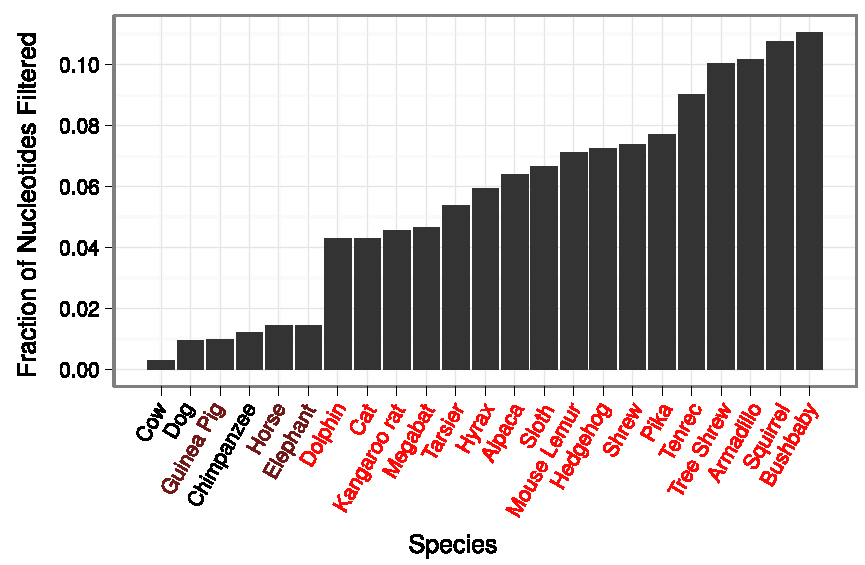
\includegraphics[scale=0.9]{Figs/qual_filter_hist.pdf}
\caption{The fraction of nucleotides masked from protein-coding
  regions of mammalian genomes based on low predicted sequence
  quality. For genomes with Phred sequence quality scores available,
  all codons containing any nucleotides with a Phred score $<25$ were
  masked with `N's. Each bar shows the fraction of nucleotide
  sequences (compared to the total number of coding nucleotides from
  each genome) which were masked. As in Figure \ref{fig_ncbi_tree},
  high-coverage genomes are labeled in black, \lcv genomes are labeled
  in red, and guinea pig and elephant---whose genomes were originally
  sequenced at 2x coverage but were later ``topped up'' to 7x
  coverage--are labeled in dark red. Phred scores were unavailable for
  most high-coverage genomes, and Phred scores for wallaby were unable
  to be used due to mismatched assembly versions (see text).}
\label{filtered_qual_bars}
\end{figure}

The above filtering scheme was applied to all coding sequences from
each genome for which quality scores were available, which included
all of the \lcv genomes (except for wallaby) and six high-coverage
genomes. Unfortunately, the \lcv wallaby genome was not filtered based
on sequence quality due to a mismatch in the sequence identifiers used
by \ens and those found in the quality score files made available for
download; wallaby was not one of the 29 species included in the
original \ac{mgp} analysis, but this error has been marked for
correction in a future version of the 38-species analysis. Note also
that the guinea pig, rabbit, microbat, horse and elephant genomes were
originally sequenced at low 2x coverage for the \ac{mgp}, but they
since underwent additional sequencing to produce high-coverage 7x
assemblies (these species are labeled in dark red in Figure
\ref{fig_ncbi_tree} from Chapter \ref{ch_orthologs}). These
higher-coverage assemblies were used for release 63 of \ens and for
the present analysis. Phred scores for the high-coverage guinea pig,
horse, and elephant assemblies were used for filtering here, but Phred
scores for the high-coverage rabbit and microbat assemblies were not
provided by the sequencing institutions.

The fraction of nucleotides filtered from each genome is shown in
Figure \ref{filtered_qual_bars}. Genomes with high-coverage assemblies
contained fewer bases with low Phred scores, resulting in 1-2\% of
nucleotides being filtered, while the bulk of low-coverage genomes
resulted in 4-8\% of nucleotides being filtered.  Five genomes
(bushbaby, squirrel, tree shrew, armadillo and tenrec) showed a
noticeably higher proportion of low-quality bases, with 9-11\%
nucleotides being filtered out. The distribution of filtered
nucleotide proportions confirmed the expectation based on
\citet{Hubisz2011} that 5-10\% of nucleotides would be filtered using
a Phred score threshold of 25, and the variation in filtered
nucleotide proportions between different \lcv species showed that
despite the uniform 2x coverage of the \lcv mammalian genomes,
different assemblies varied widely in their distributions of sequence
quality scores within coding regions.

The lack of publicly available sequence quality scores for most
high-coverage genomes was lamentable, especially for the
closely-related primates. Taking chimpanzee as an example
high-coverage genome with quality scores available (although it may
have an exceptionally error-prone genome sequence
\citep{Mallick2009}), the procedure described above resulted in
331,737 nucleotides, or roughly 1\% of all protein-coding nucleotides,
being masked. Clearly some of those masked nucleotides were of lower
quality and some were of higher quality (i.e., high-quality
nucleotides removed on account of being within a masked codon). But if
one assumes a constant error probability among masked nucleotides of
$3.16e-3$ (corresponding to the $Q=25$ threshold), then an expected
1,049 of the masked chimpanzee nucleotides contained sequencing
errors. An equivalent calculation for bushbaby, a \lcv primate genome,
yielded 2,694,054 filtered nucleotides and 8,519 expected sequencing
errors.

These numbers may be evaluated in terms of signal and noise, where
true substitution events are the desired evolutionary signal and
errors are noise. To estimate the amount of ``signal'' present in each
species' terminal lineage, the genome-wide set of filtered alignments
was used to infer substitution events along each branch (the methods
used for this are described in Section
\ref{section_windows_clustered_subs}), yielding 85,368 substitutions
along the chimpanzee branch and 892,890 substitutions along the
bushbaby branch. Comparing the inferred signal to the estimated noise
in each of these example genomes, one finds that for each true
lineage-specific substitution there were approximately 0.0095 expected
errors in the bushbaby genome and 0.0123 expected errors in the
chimpanzee genome. Thus, even though the chimpanzee genome was
sequenced to 6x coverage while bushbaby was only sequenced to 2x
coverage, the unmasked chimpanzee genome contained perhaps a lower
``signal-to-noise'' ratio within coding sequences than the unmasked
bushbaby genome.

These calculations were in general agreement with a study by
\citet{Taudien2006} which appraised the extent to which errors in an
earlier \ac{wd} version of the chimpanzee genome affected the
comparative analysis of coding regions. Although the overall error
rate of the \ac{wd} sequence was low, they found that up to 20\% of
the exonic sequence differences between human and chimpanzee were
false positives resulting from errors in the chimpanzee sequence. When
a quality score threshold of $Q>20$ was used, however, the proportion
of false positives decreased markedly to 8\% \citep{Taudien2006}. The
issue of sequence quality will be considered again in Chapter
\ref{ch_gorilla}, where I examined the impact of sequence filtering on
the estimation of genome-wide \dnds values within primates.

\subsection{Removing recent paralogs}
\label{sec_removing_paralogs}

%As discussed in Section \ref{section_quantifying_paralogous}, 

Chapter \ref{ch_orthologs} discussed a number of issues relating to
the identification of homologous protein-coding sequences, and a set
of largely orthologous gene trees was collected. The relatively low
amount of sequence divergence within mammals suggested that the
probability of erroneous inclusion of altogether non-homologous
sequences was low, but the existence of paralogous relationships
within the alignments used for \sw analysis was still a concern.

\bresp{Duplicated Genes}

Although the identification and analysis of adaptive evolution
following gene duplication is of great interest
\citep{Lynch2000,Zhang2002,He2005,Hahn2009a}, duplicated genes are
complex to analyze, in part because the presence of duplications in a
gene family affects the structure of the phylogenetic tree relating
that family's member genes. Furthermore, the inclusion of paralogous
gene relationships in a large-scale analysis of orthologous gene
evolution may produce unwanted signals of adaptive evolution following
gene duplication \citep{Lynch2000}, artifacts resulting from gene
conversion \citep{Casola2009} or biases due to lineage-specific family
expansion, a process which is relatively common in mammalian gene
families \citep{Gu2002}.

\eresp{Duplicated Genes}

As a result, it has traditionally been considered important to filter
out recently-duplicated genes (e.g., genes duplicated after the
whole-genome duplication event in the vertebrate ancestor) in
large-scale evolutionary analyses. Previous genome-wide scans for
positive selection involving six or fewer mammalian genomes have
either required strict one-to-one orthology
\citep{Clark2003,Nielsen2005} or allowed very limited numbers of
recent duplications in specific lineages \citep{Kosiol2008}. With
larger numbers of species included in a phylogenetic analysis,
however, the requirement of strict one-to-one orthology becomes
increasingly untenable: if gene duplications and deletions occur
randomly in time, then the probability of observing at least one such
event in a given gene family should increase linearly with the amount
of branch length covered by the tree. The requirement of one-to-one
orthology would result in fewer genes being available for analysis as
more species are included, which is clearly an undesirable trend. As
an alternative to ignoring genes which do not satisfy the requirement
of strict orthology, I developed an approach, described below, for
handling recently duplicated genes by removing the more divergent or
shorter paralogous copy from the gene tree.

%Before describing the method for duplications, it is worth making a
%point about gene deletions. Specifically, I note that gene deletions
%can complicate the branch-specific detection of positive selection,
%but they should not have a detrimental effect on tests for selection
%across the entire tree. The effect on branch-specific tests results
%from the merging of multiple ancestral branches into one. Take for
%example the inference of mutations along the evolutionary tree of
%human, chimpanzee and gorilla, which contains two internal nodes:
%$HC$, the human-chimpanzee ancestor, and $HCG$, the
%human-chimpanzee-gorilla ancestor. When sequences from all species are
%present, mutations can be separately identified as occurring along the
%branch from $HCG$ to $HC$ and along the branch from $HC$ to the human
%sequence, allowing for a test to differentiate between a signal of
%adaptive evolution in one branch or the other. For a gene which was
%deleted in chimpanzee those two branches become effectively merged
%into one, and mutations can only be inferred to have occurred between
%$HCG$ and the human sequence. The time-specificity of estimated
%evolutionary rates is thus reduced, and when the identity of the
%branch along which \syn and \nsyn mutations have occurred is important
%to a test for positive selection, this difference can complicate the
%interpretation of results. Acknowledging this effect,
%\citet{Kosiol2008} used a different set of orthology requirements for
%each branch-specific test for positive selection performed. When the
%test for positive selection does not depend on the identity of
%specific branches in the tree, however, a gene deletion would only
%serve to reduce the total amount of branch length available for
%inference. As long as the branch leading to the deleted species did
%not comprise a large portion of the total branch length, the effect of
%gene deletion on the results of tree-wide tests for selection should
%be minimal.

%Turning back to gene duplications,

An additional complicating factor in the current analysis was the
concern that many of the apparent gene duplications might actually be
artifacts of the annotation of \lcv genomes. Each \lcv genome assembly
is highly fragmented, meaning that it contains many short sequence
segments that were unable to be assembled into chromosome-sized
sequences due to missing intervening sequence data. Sometimes the
exons of a gene spanned the boundaries of these sequence segments,
causing different parts of a gene to exist on different segments. The
\ens annotation pipeline was not designed to merge gene annotations
across different sequence segments, so each part of a gene residing on
multiple sequence segments would be annotated as a separate shortened
gene. These shortened genes would be treated as independent proteins
by the \cmp pipeline, likely being placed at very similar positions in
the gene tree due to each sequence having been derived from a gene
with a single correct evolutionary position. This result might not be
detrimental to sitewise analysis in itself, as each shortened gene may
end up being correctly aligned and provide useful information to the
alignment. However, a number of factors, including the low quality of
genomic sequence and assembly within these shortened genes, problems
with aligning small fractions of a gene against complete sequences and
the potential for incorrect placement of fragmented sequences within
the gene tree, made it desirable to remove the shortest of these gene
fragments.

Sequence divergence was the other criterion used to select which
paralogous copy of recently-duplicated genes to retain. Models of
evolution after gene duplication have tended to predict that one of the
duplicate copies retains the ancestral function (and its associated
pattern of evolutionary constraint) while the other duplicate
experiences relaxed constraint followed by either degradation or
functional diversification \citep{Han2009}. Thus, the least-diverged
copy of a recently duplicated gene should be the one most likely to
have retained the pattern of evolutionary constraint shared among the
mammalian species being examined in this study.

The protocol I implemented for filtering apparent paralogs used both
gene length and sequence divergence to identify which gene among a set
of apparent paralogous copies was most suitable to retain for
analysis. Gene length was used primarily to discriminate spuriously
shortened genes from true genes, and sequence divergence was used to
distinguish between more- and less-diverged paralogs. First, the mean
pairwise sequence distance was calculated between each putative
paralog and all other sequences in the gene tree, resulting in one
mean pairwise distance estimate per putative paralog (hereafter
referred to as the mean distance). For these distance calculations,
the coding sequence alignments provided by \ens \cmp and the JC69
nucleotide model were used to estimate distances. Second, the ratio of
the sequence length of each putative paralog to the mean sequence
length across the tree (hereafter referred to as the length ratio) was
also calculated.

Genes were grouped by species within each gene tree, and any group of
two or more genes from the same species was considered to be a set of
putative paralogs. Within each set of putative paralogs, a single gene
was chosen to be retained for evolutionary analysis based on three
rules applied in the following order: (1) if only one sequence had a
length ratio above 0.5 and all others had a length ratio below 0.5,
the longest sequence was kept; (2) if one sequence yielded a mean
distance below the others, that sequence was kept; (3) if all mean
distances were identical then the longest sequence was kept, or if all
mean distances and length ratios were equal, an arbitrary choice was
made.

\begin{figure}
\centering
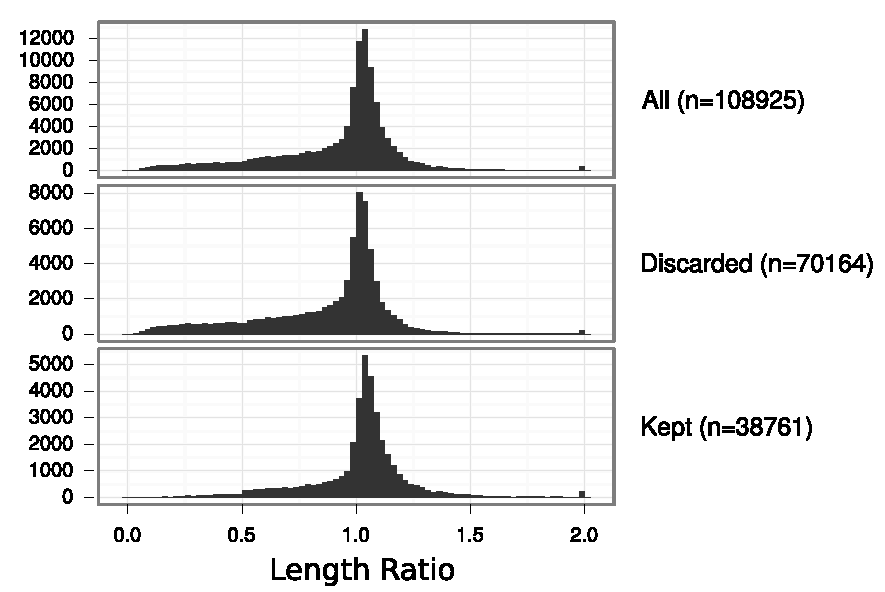
\includegraphics[scale=0.9]{Figs/mammals_paralogs_hist.pdf}
\caption{Length ratios of putative paralogs. The length ratio was
  calculated as the length of a putative paralogous copy divided by
  the mean length all sequences its corresponding gene
  tree. Putatively paralogous genes (top panel) were either discarded
  (middle panel) or kept (bottom panel) according to rules based on
  their length and mean sequence divergence from other aligned
  sequences, as described in the text.}
\label{filtered_paralogs_hist}
\end{figure}

These rules were applied to each of the 108,925 putative paralogs
within the 9,604 gene trees containing at least one set of putative
paralogs. Figure \ref{filtered_paralogs_hist} shows the distributions
of length ratios for the set of all putative paralogs, those discarded
from the alignments, and those kept for subsequent analysis. The
overall distribution of length ratios showed that most putative
paralogs had lengths similar to the mean length across the gene tree
(with a peak at or slightly above 1), but the shape of the
distribution was asymmetric, with a bias towards shorter lengths. The
filtering protocol effectively removed these shortened genes, as
evidenced by the enrichment of lower length ratios in the distribution
of discarded genes and the less skewed distribution of length ratios
in the set of 38,761 retained putative paralogs.

\begin{figure}
\centering
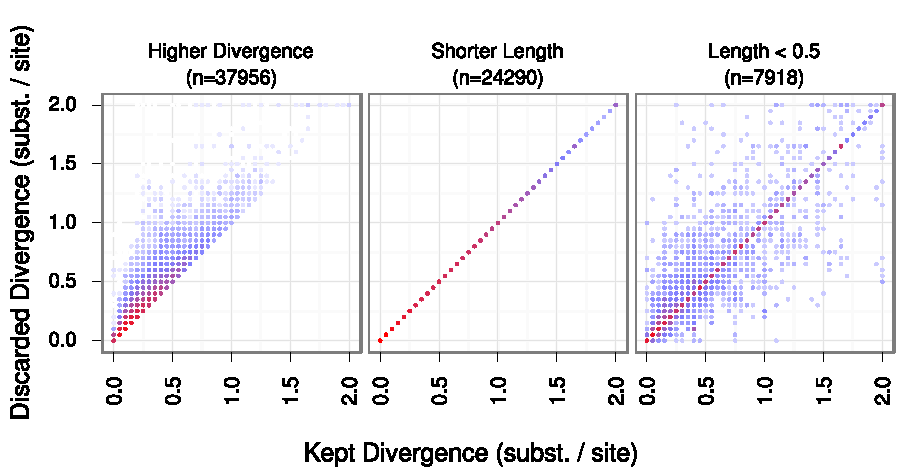
\includegraphics[scale=0.9]{Figs/mammals_paralogs_scatter.pdf}
\caption{Sequence divergence of retained and discarded putative
  paralogs. Each data point was a gene which was discarded from the
  tree for one of three reasons: it had a length ratio of less than
  0.5 while the retained copy had a length ratio greater than 0.5
  (\emph{Length $<0.5$}; right panel), it had more sequence divergence
  than the retained gene (\emph{Higher Divergence}; middle panel), or
  it had equal sequence divergence but shorter length than the
  retained gene (\emph{Shorter Length}; right panel). Divergence was
  measured as the mean pairwise divergence between the gene and all
  other sequences in the tree. Each colored point represents the
  binned density of sites; no points are drawn where no density
  exists, while blue and red points are drawn at areas of low and high
  density, respectively.}
\label{filtered_paralogs_scatter}
\end{figure}

A more detailed view of the results of the paralog filter is presented
in Figure \ref{filtered_paralogs_scatter}, showing a scatter plot of
the mean distance and length ratio of each discarded paralog compared
to that of the corresponding kept paralog. Figure
\ref{filtered_paralogs_scatter} is separated into panels according to
the rule used to discard the paralogous copy: the first panel
corresponds to rule (1), where genes with a length ratio below 0.5
were discarded; the second panel corresponds to rule (2), where genes
with higher mean distances were removed; the third panel corresponds
to rule (3), where all genes had equal mean distances and the longest
gene was kept (or, if all lengths were equal, an arbitrary choice was
made).

The first panel of Figure \ref{filtered_paralogs_scatter} shows that
genes discarded on the basis of having a very short length contained
sequence distances similar to the kept copies, as the highest density
is along the diagonal and there is perhaps only a slight bias towards
genes lying above the diagonal (i.e., in the direction of greater
divergence in the discarded copy). This was in line with the
expectation that these discarded genes were not truly paralogous
copies, but rather fragments of split genes resulting from unassembled
sequence segments. The second panel shows that when paralogous copies
could be differentiated by their mean distances, they tended to have
low average distances ($<$0.5 substitutions per nucleotide site) and
only a small difference between the kept and discarded copy (e.g.,
most of the distribution is just above the diagonal, and few points
are above the dashed line with a slope of 2). Finally, the
distribution of length ratios and mean distances in the set of genes
where length was the discriminating factor (or where an arbitrary
decision was made) shows that most of these genes were mostly
identical whether measured by sequence distance or by sequence length.

These results provided evidence that a sizeable fraction of recently
duplicated mammalian genes are identical or very similar to each
other: for roughly 30\% of all putative paralogs, not enough time has
elapsed since the duplication event for a detectable amount of
sequence change to have occurred, and the choice between retaining one
copy or the other was essentially arbitrary. For the roughly 40\% of
putative paralogs where differences in mean distance could be
identified, these differences tended to be small.

This was obviously not the most conservative approach to dealing with
recent duplications. One could instead remove all putatively
paralogous copies from the gene tree, creating an apparent gene
deletion in that species, or simply ignore all gene families with any
recent duplications (e.g., require one-to-one orthology allowing for
gene deletions). The latter option would likely be overly restrictive
for any sensible genome-wide analysis, but the former option may be
appropriate for a more conservative approach. As the main concern over
the handling duplicated genes has been that they may introduce a bias
towards elevated evolutionary rates, I marked the genes containing
sets of putative paralogs for further evaluation. Sitewise estimates
from these genes were excluded from the most conservatively-filtered
sitewise dataset and examined separately for excess signal of positive
selection (see Section \ref{section_sitewise_filtering})
%, and in the
%next chapter I examine whether using the more conservative approach of
%removing all paralogous copies from genes removed the signal of
%positive selection from a subset of genes (see Section
%\ref{section_genes_paralog_subset}).

\subsection{Identifying clusters of \nsyn substitutions}
\label{section_windows_clustered_subs}

After filtering for sequence quality and removing paralogous genes and
shortened gene fragments, \prankc was used to align the codon
sequences of each of the \ntrees mammalian gene trees. Manual analysis
of a number of these alignments revealed many short stretches of
clearly nonhomologous sequence in one species, often flanked by
stretches of perfect homology and often lying on the borders of exon
junctions. Examples of two such regions are shown in Figure
\ref{fig_mammals_cluster_subs}.  These obviously erroneous stretches
were likely due to mis-assembly of a genomic region or
misidentification of exon boundaries within the gene of one
species. In the examples in Figure \ref{fig_mammals_cluster_subs},
most of the nonhomologous material was inferred to be a
lineage-specific insertion in the mis-annotated species; these regions
were not of concern, as \ac{slr} ignores single-species insertions
because they contain no evolutionary information. More concerning,
however, were the regions indicated with red brackets in Figure
\ref{fig_mammals_cluster_subs} where the apparently \nhom material was
aligned with other species. These regions were particularly concerning
with respect to the detection of positive selection, as the
incorporation of a stretch of apparently nonhomologous material into a
sequence alignment would produce many alignment columns with multiple
nucleotide differences per codon. As discussed in Section
\ref{sec_error_impact}, this type of error is particularly prone to
cause false positives in the detection of positive selection.

\begin{figure}
\centering 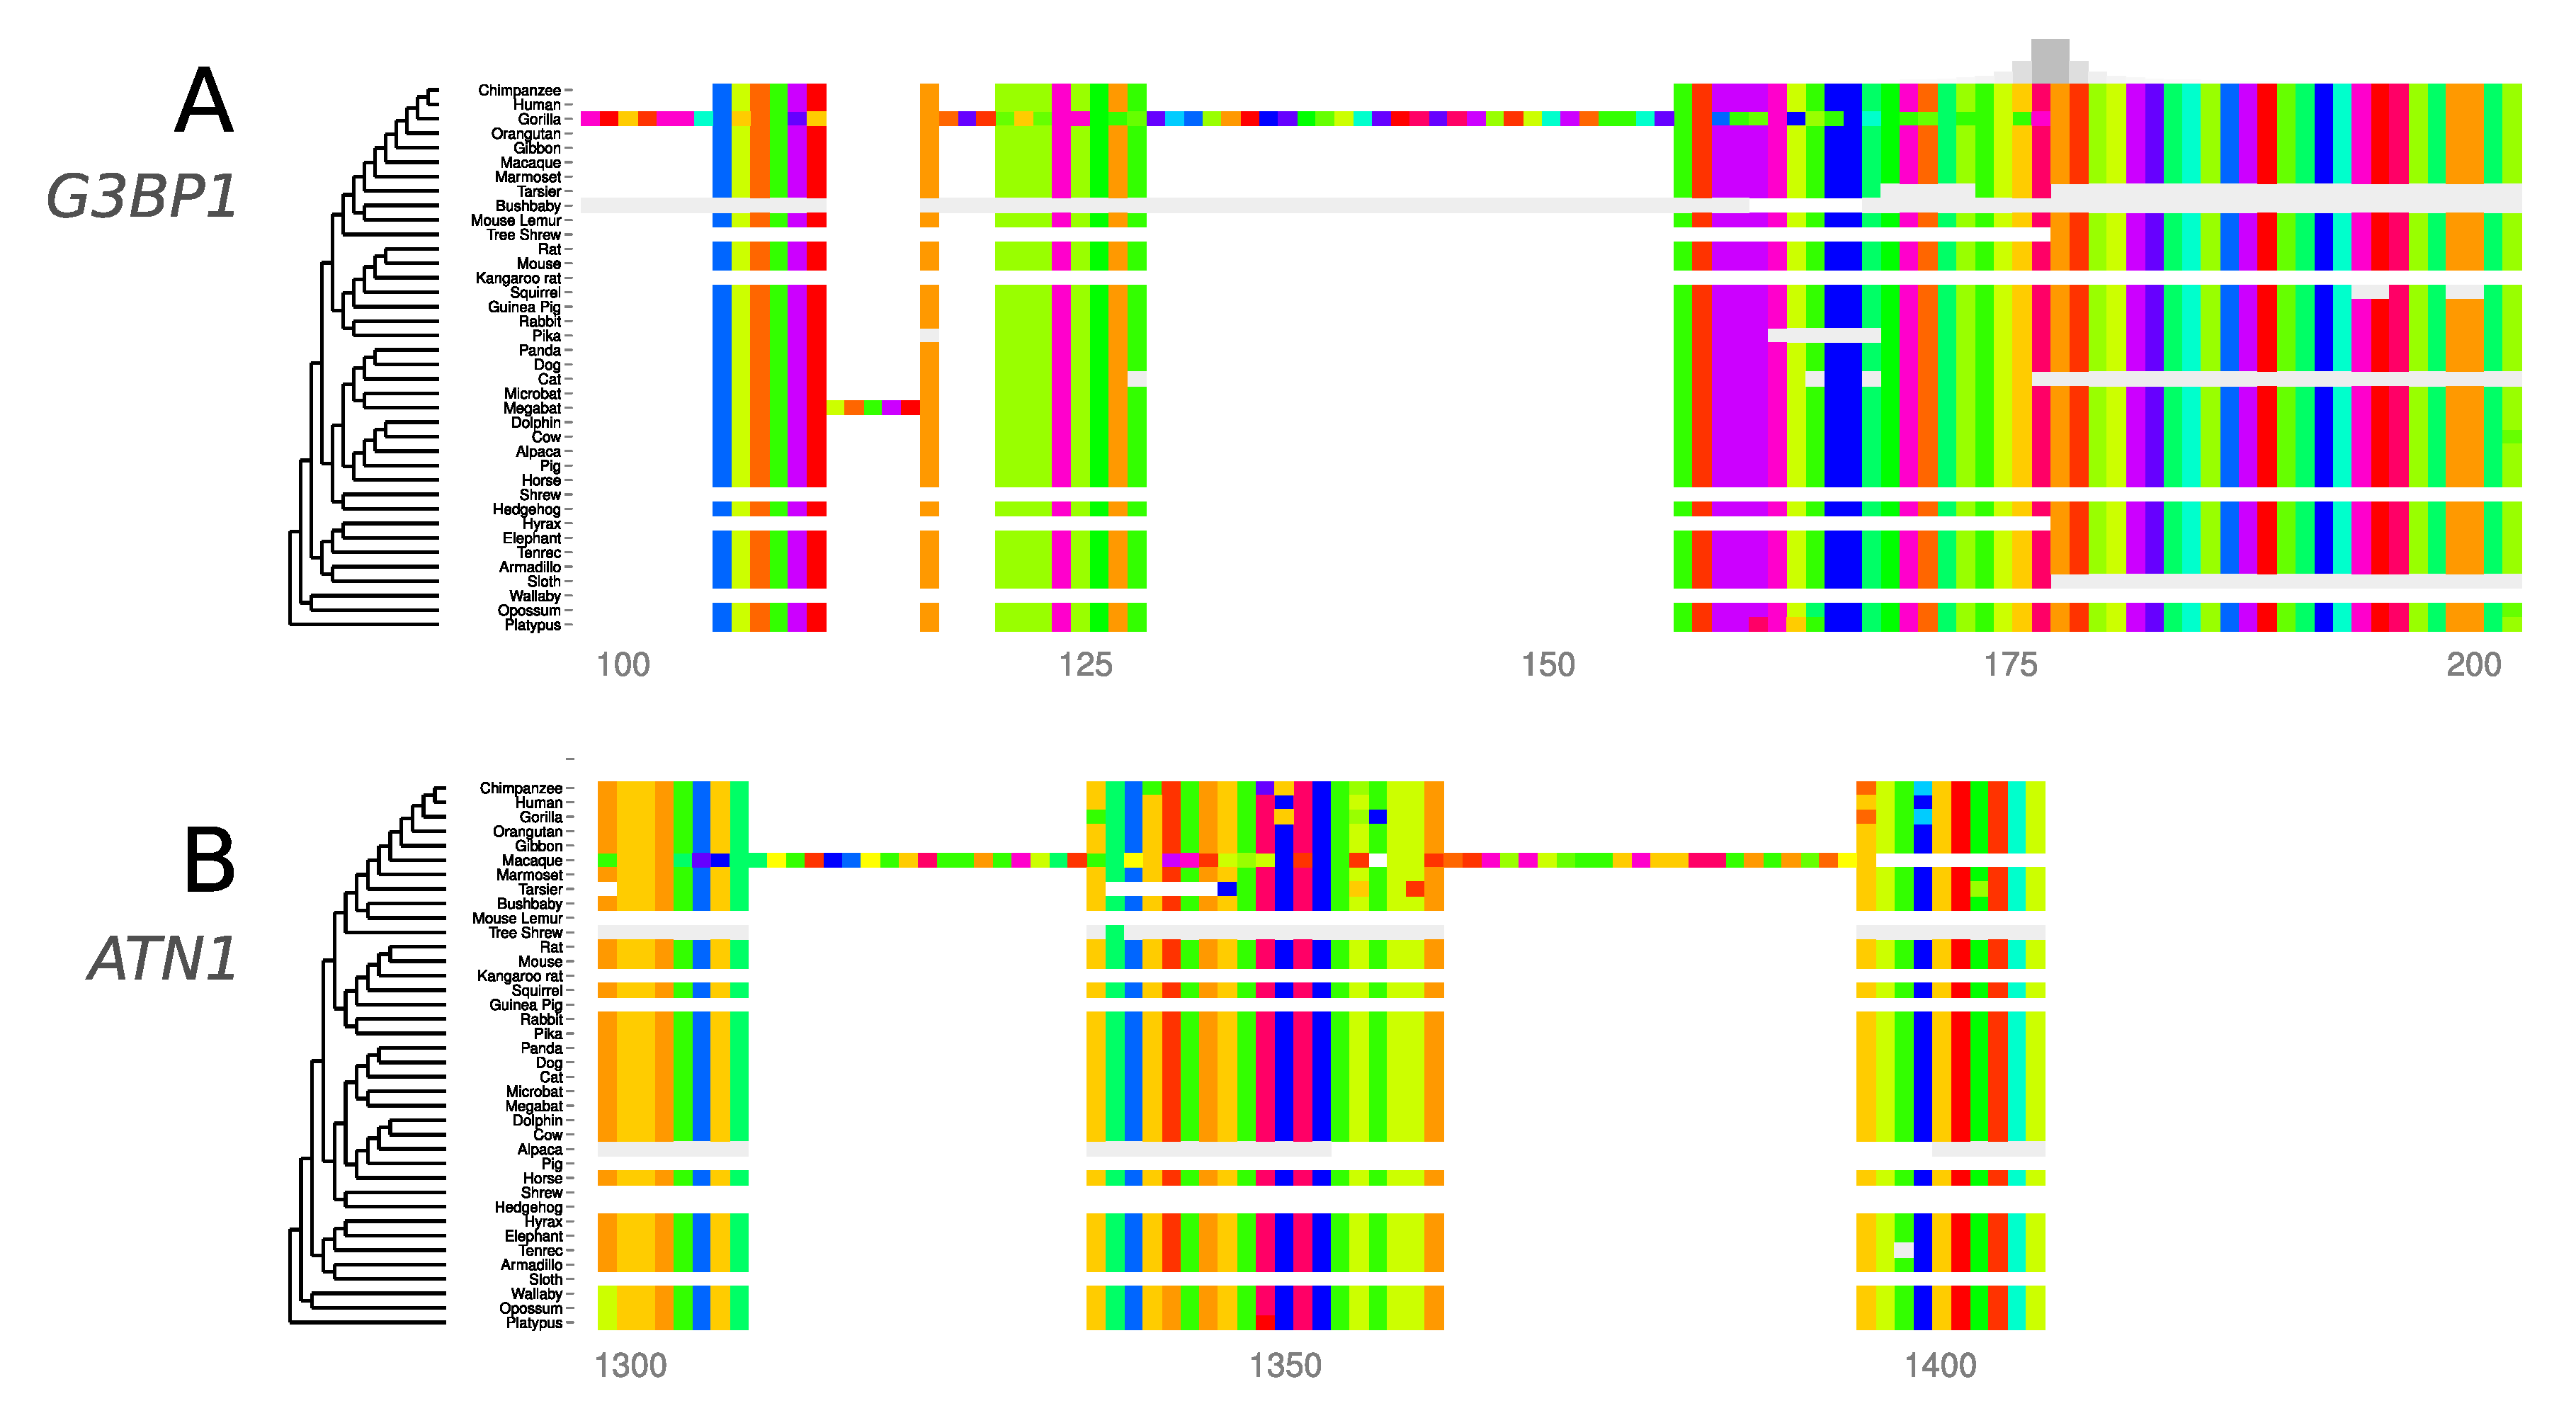
\includegraphics[scale=0.25]{Figs/mammals_cluster_subs.pdf}
\caption{Two regions of protein-coding mammalian alignments with
  stretches of \nhom sequence in one species. Alignments are shown
  with amino acids colored according to \citet{Taylor1986}. (A) The
  \gene{G3BP1} alignment, showing a mis-annotated exon in gorilla
  resulting in misalignment. (B) The \gene{ATN1} alignment, showing a
  mis-annotated exon in macaque resulting in misalignment. The regions
  indicated by red brackets contained aligned \nhom material that
  might cause false positives in detecting \sw positive selection.}
\label{fig_mammals_cluster_subs}
\end{figure}

I hypothesized that these stretches of \nhom sequence could be
identified by their impact on the pattern of substitutions within each
alignment. A stretch of \nhom aligned sequence would be expected to
produce a localized cluster of apparent synonymous and nonsynonymous
substitutions occurring along the branch between the sequence
containing the erroneous stretch and its ancestor. Because these
substitutions would be restricted to one terminal branch in the gene
tree and a region of the alignment limited to the length of the \nhom
stretch, a scan for clustered substitutions within the terminal
lineages of genes might be an effective way of identifying these
erroneous sequences.

Two factors could confound the effectiveness of using clustered
substitutions to identify regions of \nhom aligned sequence. First,
the length of the terminal branch leading to each species determines
how many lineage-specific substitutions would be expected to occur
within a window of a certain size. The terminal human branch, for
example, is very short, while the platypus branch is very long. Thus,
one would expect to observe many more lineage-specific substitutions
in platypus than in human for a given alignment window. In contrast, a
stretch of \nhom aligned sequence should introduce, on average, a
constant number of \nsyn and \syn substitutions into the branch
ancestral to the sequence in which it exists. For this reason it
should be more difficult to distinguish homologous from \nhom
stretches in species with long terminal lineages. On the other hand,
this trend should also serve to limit the negative impact of \nhom
stretches in those species on the detection of positive selection,
because the resulting elevation in \nsyn or \syn substitutions rates
would be less severe.

The second confounding factor is that \nsyn substitutions have been
shown to be significantly more clustered than expected by chance in a
number of genomic analyses of mammalian and insect genomes
\citep{Callahan2011,Bazykin2004,Wang2007}. Thus, a filter based on
clustered \nsyn substitutions may have a tendency to remove true
clusters of \nsyn substitutions from the dataset. The influence of
this factor may be evaluated by comparing clusters of substitutions in
terminal branches to those in internal branches: while both internal
and terminal branches of the mammalian tree should harbor similar
levels of truly clustered \nsyn and \syn substitutions, only the
terminal lineages should contain large clusters resulting from
stretches of aligned \nhom sequence.

I investigated the distributions of \nsyn and \syn substitutions
within windows of mammalian alignments by using \emph{codeml}
\citep{Yang2007} under the M0 model (e.g., assuming one \omg for
all sites and all branches in the tree) to perform the marginal
reconstruction of ancestral sequences at internal nodes
\citep{Yang1995} and to identify the substitution events implied by
the reconstructed ancestral sequences of each gene alignment. Only
substitution events occurring between codons with high posterior
probabilities in the marginal ancestral reconstruction ($>0.9$) were
analyzed, and the location of each substitution event along the
alignment and within the gene tree was stored. This analysis was
performed on all gene trees, yielding a large database of confidently
inferred substitution events along internal and terminal branches of
the mammalian phylogenetic tree.

Counts of \syn and \nsyn substitutions along each branch were
separately collected for non-overlapping 15-codon alignment windows;
the results for a selection of species and internal nodes are shown in
Figure \ref{fig_wcs}, which plots the number of 15-codon windows
containing a given number of \nsyn and \syn substitutions for a
selection of terminal and internal nodes. Each window is thus
represented twice in Figure \ref{fig_wcs}: once in the \nsyn
histogram, and once in the \syn histogram. Windows with no
substitutions along the given branch are represented in the left-most
\syn and \nsyn bins. The mean length of the branch ancestral to the
given node, calculated from the set of branch lengths estimated by
\emph{codeml}, is indicated in parentheses after each node name.

\begin{figure}
\centering 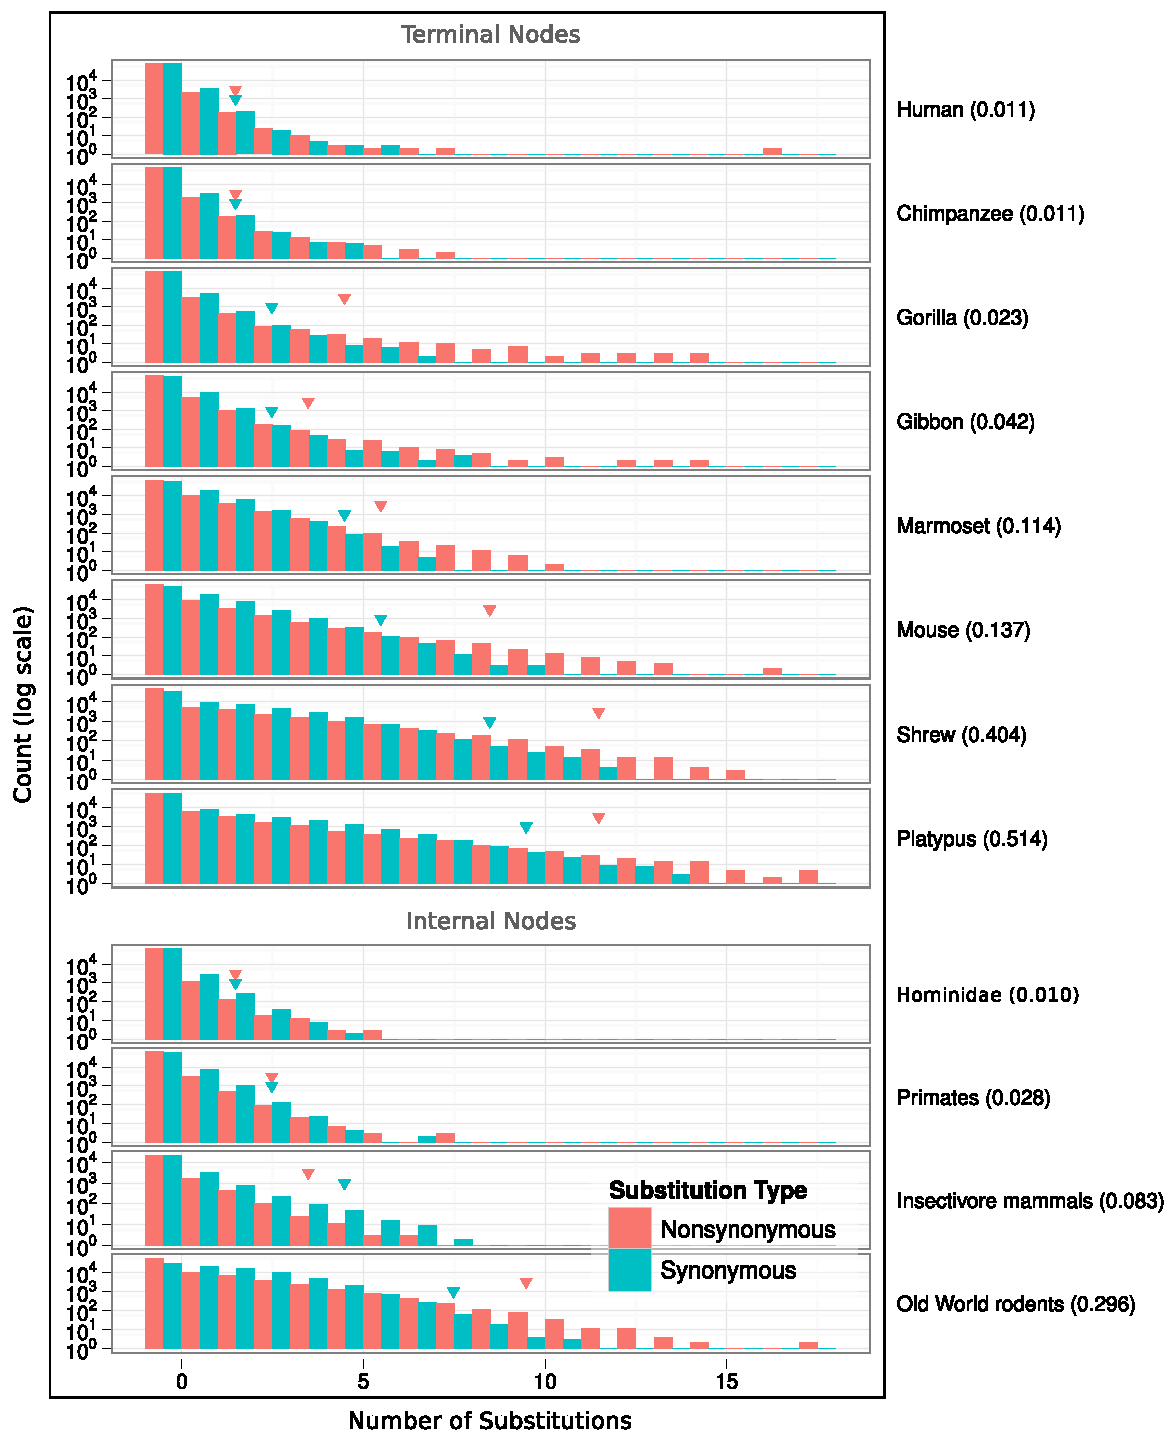
\includegraphics[scale=0.75]{Figs/wcs_15.pdf}
\caption{Counts of inferred \nsyn (red bars) and \syn (blue bars)
  substitutions in 15-codon windows along terminal and internal
  branches of the mammalian tree. The leftmost two bars correspond to
  windows with 0 substitutions, the next two bars correspond to
  windows with 1 substitution, and so on. Red and blue arrows indicate
  the number of \nsyn and \syn substitutions, respectively,
  corresponding to the 99.9\% percentile across all windows in that
  node. The mean length of the branch ancestral to each node is
  included in parentheses after the node label.}
\label{fig_wcs}
\end{figure}

Figure \ref{fig_wcs} shows that the vast majority of 15-codon windows
in these alignments contained few substitutions (note that the
$y$-axis uses a logarithmic scale), but a long tail of \nsyn and \syn
substitutions were observed for some nodes. Comparing the counts of
\nsyn vs.\ \syn substitutions within the terminal nodes (Figure
\ref{fig_wcs}, top panel), a pattern is seen where the \nsyn counts
(red bars) are higher than \syn counts at 0 substitutions, lower than
\syn counts in the middle range of substitutions (1--5 substitutions),
and higher again in the higher range of substitutions ($>$5
substitutions). The pattern in the lower range is consistent with the
action of purifying selection on protein-coding regions, causing a
reduced number of windows with multiple \nsyn substitutions compared
to \syn substitutions. The excess of windows with large numbers of
\nsyn substitutions, on the other hand, runs against the pattern of
purifying selection; instead, it shows unexpectedly long clusters of
\nsyn substitutions to be a widespread feature of these mammalian
alignments. The red and blue triangles drawn in each plot mark the
number of substitutions below which 99.9\% of windows are contained;
the shift of the \nsyn markers to the right in most of the terminal
branches emphasizes the excess of highly clustered \nsyn
substitutions. Interestingly, human---which has the highest quality
and best annotated genome---does not show the same level of excess
seen in the other genomes analyzed.

Comparing the pattern seen for terminal nodes to those from internal
nodes provided further evidence for the presence of many stretches of
\nhom sequence within the mammalian alignments. For example, the
terminal gorilla node is roughly equivalent in average branch length
to the internal primates node ($0.023$ vs.\ $0.028$), but gorilla
contains windows with up to 14 \nsyn substitutions while primates
contain a maximum of 8. Looking at the \nsyn and \syn 99.9\%
quantiles, three of the four internal nodes had equal or lower
quantile positions for \nsyn versus \syn substitutions, but the rodent
ancestral node showed a pattern more similar to the terminal nodes in
Figure \ref{fig_wcs}, with a higher 99\% quantile for \nsyn
substitutions. This was an interesting difference, as the gene
annotations for most rodent genomes were likely derived from
alignments to mouse rather than human. In the case of discordant gene
annotations, the entire rodent clade would share an aligned \nhom
stretch, causing clustered substitutions to be inferred along the
internal rodent branch. This raised the possibility that the entire
rodent clade contains many misaligned \nhom stretches due to shared
differences in gene annotations between rodent and non-rodent species.


\bresp{Window Size}

Window sizes of 8 and 30 codons were also tested using the same
approach; the data are not shown here, but the results were
qualitatively similar. Visual inspection of several problematic
alignments showed that the nonhomologous aligned sequence was often
between 10-20 codons in length, so a 15-codon window seemed to be the
size best suited for detecting these problematic regions. Smaller
windows might suffer from decreased specificity, as non-erroneous
alignments might reasonably contain very small clusters of
nonsynonymous substitutions. Too large a window size could yield
reduced sensitivity, because a given window might extend beyond a
given stretch of nonhomologous aligned sequence, resulting in a mix of
nonhomologous and homologous sequence contributing to the substitution
counts.

\eresp{Window Size}

%This appeared to be the case for at least one gene: Figure
%\ref{fig_mouse_crap_aln} shows the region surrounding a 15-codon
%window with 11 apparent rodent \nsyn substitutions, likely the result
%of a difference in exon annotations between rodent and non-rodent
%genomes.

The end result of this analysis was the identification, for each
terminal node of the mammalian tree, of windows with \nsyn
substitution counts above the top 0.1\% of 15-codon windows; these
windows were considered potential stretches of \nhom aligned
sequence. Despite evidence that some internal nodes might also suffer
from this type of alignment artifact, most internal nodes were free
from an obvious excess of clustered \nsyn substitutions, so internal
nodes were excluded from this list. A qualitative analysis of regions
containing windows at a variety of thresholds found the 0.1\%
threshold to strike a good balance between sensitivity and
specificity.

In total, 37,824 windows containing potential stretches of \nhom
aligned sequence were identified across 8,951 alignments, with 881
genes containing more than 10 windows each. The locations of these
windows were stored for later use in defining the most
conservatively-filtered sitewise dataset.

%\section{Genome-wide analysis of sitewise selective pressures in mammals}

\section{Species groups for sitewise analysis}

% latex table generated in R 2.13.0 by xtable 1.5-6 package
% Thu Sep 15 11:19:59 2011
\begin{table}
\centering \footnotesize
\begin{tabular}{lrb{8cm}rr}
\toprule
 & \multicolumn{2}{c}{Species} & \multicolumn{2}{c}{Median dS} \\
\cmidrule(r){2-3} \cmidrule{4-5}
Name & Count & List & MPL & Total \\
  \midrule
\input{Tables/table_species_set_summary.txt}
\bottomrule
\end{tabular}
\caption{Species groups used for sitewise analysis by \ac{slr}. The
  median \acp{mpl} and the median total branch length are shown for
  each species group, taken from the \ntrees branch lengths estimated
  by \ac{slr} for each gene. MPL -- mean path length.}
\label{table_species_set_summary}
\end{table}

For each alignment of mammalian orthologs, SLR was run separately on
10 different sets of mammalian species to obtain sitewise estimates in
a variety of species groups. For each species group, sequences
corresponding to species within the group were extracted from the
whole mammalian alignment (along with the corresponding \subtr) and
input to SLR, which was run with its default parameters. If fewer than
two sequences were available for a given gene and species group, the
sitewise analysis was skipped for that group. The species included in
each group are listed in Table \ref{table_species_set_summary}
alongside the \acf{mpl} and total branch length of their subtrees,
estimated as the median value across all \ntrees genes' estimates of
\ds distances.

Three of the species groups (Glires, Primates, and Laurasiatheria) were
chosen because they represent the three mammalian superorders with the
greatest taxonomic representation in Ensembl, providing an opportunity
to compare the molecular evolutionary dynamics of three monophyletic
mammalian groups containing varying levels of divergence, diverse
biological characteristics, and a number of high-quality reference
genomes. A fourth parallel mammalian subclade, Atlantogenata,
consisting of sloth, armadillo, tenrec, elephant and hyrax, was also
included, but the monophyly of this group is still under debate
\citep{Murphy2007,Churakov2009} and it contains only one high-coverage
genome. As such, it was not considered a primary target for the
mammalian superorder analysis. The different mammalian superorders
contained a wide range of total branch lengths, with 0.83 for
Primates, 0.97 for Atlantogenata, 1.90 for Glires, and 2.16 for
Laurasiatheria. A slightly different ordering was found when measuring
the trees by \ac{mpl}, with Glires having a significantly higher
\ac{mpl} (0.40) than the other groups despite having fewer species and
a lower total branch length than Laurasiatheria. This reflected the
higher neutral evolutionary rate in the Glires group, a
well-documented feature of rodent evolution likely resulting from
their long-term shorter generation time, which has been strongly
correlated with higher neutral evolutionary rates
\citep{Nikolaev2007,Smith2008}.

Two larger species groups, Eutheria and Mammalia, were chosen for the
purpose of measuring average sitewise selective pressures across
mammals as a whole. The Eutheria group consists of the union of the
mammalian superorder groups plus armadillo, and the Mammalian group
adds opossum, platypus, and wallaby for a total of 38 species. The
median total branch lengths for Mammalia and Eutheria were 8.21 and
6.43, respectively, and the \ac{mpl}s were 0.67 and 0.35.

Finally, to evaluate the impact of species choice and branch length on
the results of the \sw analysis, four additional ``sparse'' species
groups were created for comparison to the main groups of interest. The
species in the Sparse Glires group were chosen to create a group with
species from the Glires group but having a lower overall branch
length; the Sparse Mammals group was created with a similar aim,
created by selecting one species (preferably with a high-coverage
genome) from each major mammalian branch, greatly reducing the total
branch length covered but maintaining a similar evolutionary depth and
distribution of major branches within the species tree. The HQ Mammals
group was similar to the Sparse Mammals group, but elephant and the
deeper mammalian lineages were omitted (i.e., wallaby, platypus,
armadillo) in favor of only the high-coverage Eutherian genomes (i.e.,
chimpanzee, cow, horse, macaque, pig, rat). Finally, the HMRD group
consisted of human, mouse, rat, dog, and represented the type of
phylogenetic tree that was commonly analyzed early in the last decade
when only a few mammalian genome sequences were available. The HMRD
group was comparable to Primates and Atlantogenata in total branch
length, while HQ Mammals and Sparse Glires were more similar to
Glires.

\section{Evaluating and filtering \sw results}
\label{section_sitewise_filtering}

Sitewise data were collected from SLR and stored in a database for
storage and further analysis. The Mammals group, containing the
greatest total branch length of all the datasets and representing the
entire set of aligned sequences, and the Primates group, containing
the lowest overall branch length, were used as representative species
groups to perform quality-control checks on the \sw data and to guide
the curation of filtered \sw datasets for each species group.

Two genome-wide datasets were generated by processing \sw data
separately with two levels of filtering: a relaxed filter, designed to
retain much of the data while filtering out the most obviously
low-quality sites, and a conservative filter, designed to remove a
wider set of sites and genes that showed evidence for potential
misalignment or large numbers of gene duplications.

\bbfig
\centering
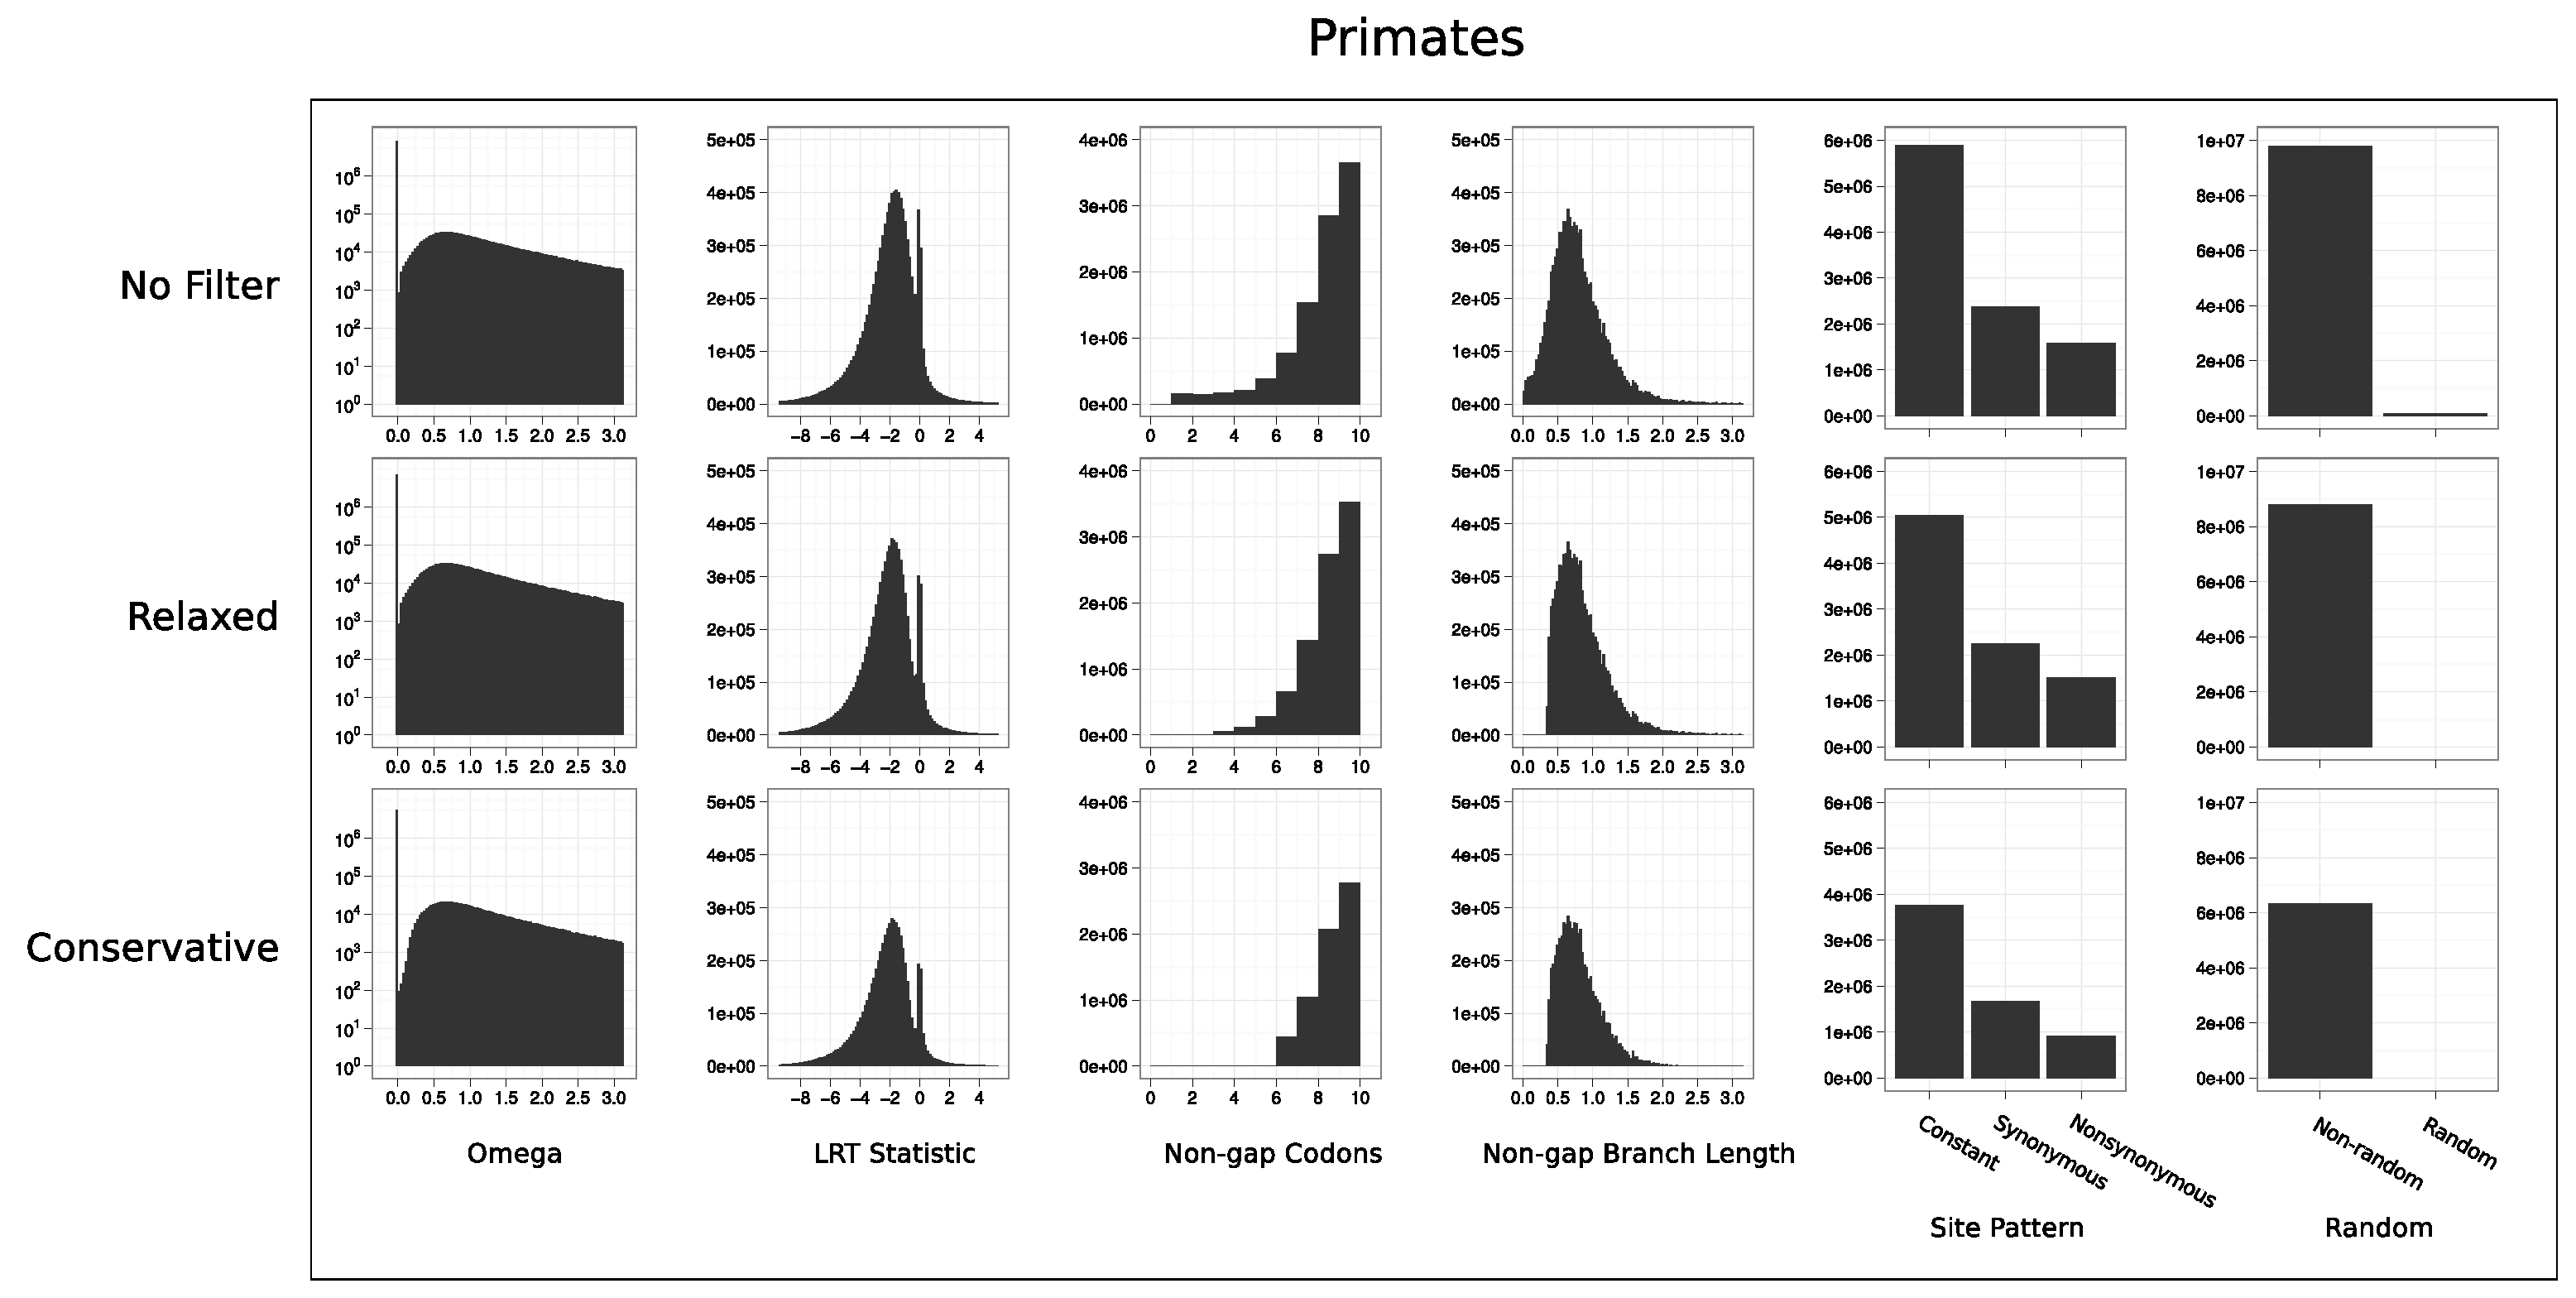
\includegraphics[scale=0.42]{Figs/qc_hist_primates.pdf}
\caption{Distributions of sitewise values for the Primates species
  group, showing the raw data (top row) and the result of applying the
  relaxed (middle row) and conservative (bottom row) filters.}
\label{fig_qc_hist_primates}
\eefig

\bbfig
\centering
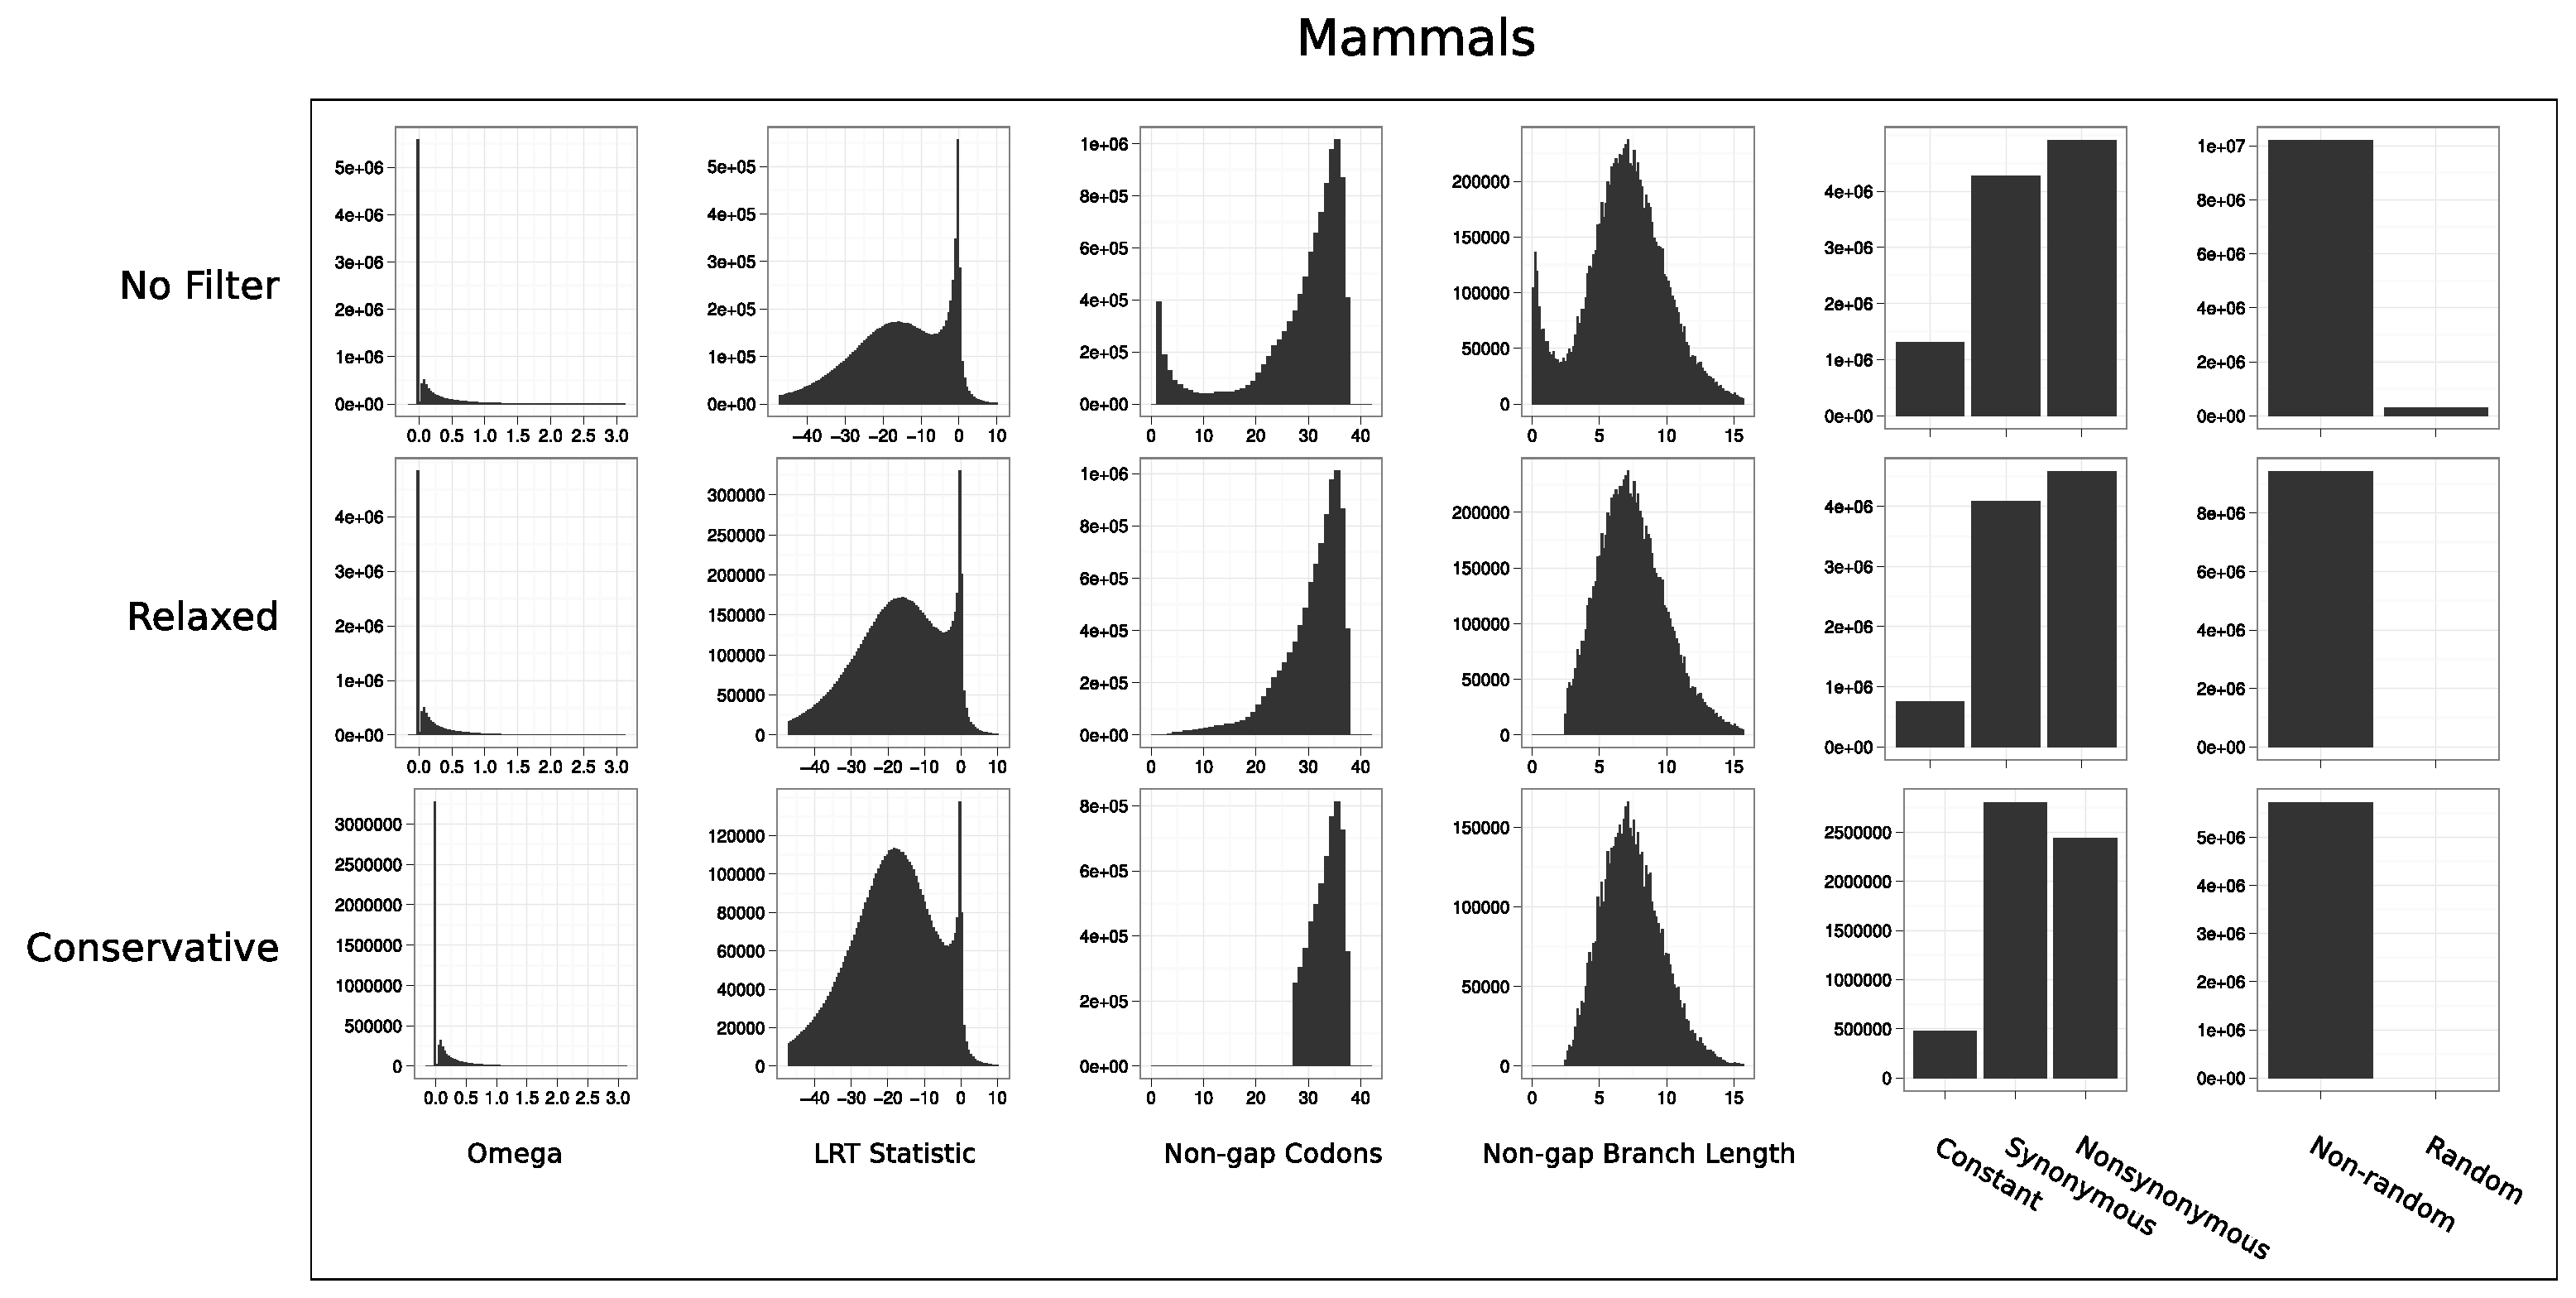
\includegraphics[scale=0.42]{Figs/qc_hist_mammals.pdf}
\caption{Distributions of sitewise values for the Mammals species
  group, showing the raw data (top row) and the result of applying the
  relaxed (middle row) and conservative (bottom row) filters.}
\label{fig_qc_hist_mammals}
\eefig
 
I first examined the overall distributions of \omg estimates and \sw
LRT statistics from SLR. Figures \ref{fig_qc_hist_primates} and
\ref{fig_qc_hist_mammals} show the distributions of six sitewise
statistics for each group of species. Four of the statistics (Omega,
LRT Statistic, Site Pattern and Random) were collected from the output
of \ac{slr} and two of the statistics (\Ngap Codons and \Ngap Branch
Length) were directly calculated from the codon alignments. The Omega
statistic is \ac{slr}'s \ac{ml} estimate of \omg, hereafter referred
to as \omgml. The LRT Statistic is the raw statistic resulting from
the \sw \ac{lrt} performed by \ac{slr}. Following Massingham
\citeyearpar{Massingham2005}, a signed version of the \ac{lrt}
statistic, hereafter \slrt, is used throughout this chapter. The \slrt
is formed by negating the raw \ac{lrt} statistic for sites where
\omgml$<1$; the signed statistic is a useful measure by which to sort
sites according to their evidence for purifying and positive
selection. The Site Pattern is a categorical classification of the
pattern of \syn and \nsyn substitutions at each site: a site is
``constant'' if it contains no differences, ``synonymous'' if it only
contains \syn differences between sequences, and \nsyn if it contains
at least one \nsyn difference. Sites designated as ``Random'' contain
a pattern of codons not significantly different from random, as
calculated by \ac{slr} based on the entropy and optimized likelihood
at that site. Finally, the \Ngap Codons and \Ngap Branch Length
statistics were calculated from the pattern of gaps and non-gaps at
each alignment column: \Ngap Codons is a count of the number of
sequences without gaps at that site, and \Ngap Branch Length measures
the total branch length of the \subtr connecting each of the \ngap
sequences.

A prominent feature of the distribution of \omgml values for the
unfiltered Mammals data, shown in the top row of Figure
\ref{fig_qc_hist_mammals}, was the large number of sites with
\omgml$=0$. Further inspection of the data revealed that all
\omgml$=0$ sites contained either \syn or constant site patterns. In
fact, all sites with constant patterns (and nearly all sites with \syn
patterns) yielded a \omgml estimate of zero. Intuitively, an estimate
of zero for \syn sites is appropriate, as the lack of any \nsyn
substitutions throughout the tree would provide no evidence for a
\nsyn substitution rate of greater than zero. For constant sites the
case is less clear, because no data regarding the rate of either \syn
or \nsyn substitutions exists in the alignment column. However, given
SLR's assumption of a constant \syn substitution rate throughout each
gene \citep{Massingham2005}, the \omg value which maximizes the
likelihood of observing zero substitutions is zero, since that value
minimizes both the \nsyn and the total substitution rate.

It is not evident from either Figure \ref{fig_qc_hist_primates} or
\ref{fig_qc_hist_mammals}, but a small proportion (ca. 0.2\%) of sites
containing \syn site patterns resulted in \omgml estimates greater
than zero. Analysis of the alignment columns corresponding to these
sites showed them all to include synonymous codons coding for serine
or arginine which are separated by multiple nucleotide
differences. Under the mechanistic codon model implemented by
\ac{slr}, which does not allow for multiple simultaneous nucleotide
changes, inferring an evolutionary path between these
multiply-substituted codons required the inference of multiple \nsyn
substitutions to reach one codon from the other. This produced a \nsyn
substitution rate of greater than zero for a site with a \syn site
pattern. The existence of multiply-substituted codons in alignments
has been previously reported \citep{Averof2000,Whelan2004}, and
empirical results have supported the notion that codon models that
allow for multiple simultaneous nucleotide changes better describe
evolution than those that do not \citep{Kosiol2007}. However, the very
low proportion of synonymous sites requiring non-zero \nsyn
substitution rates suggested that the impact of these effects on the
current dataset was minimal; this was likely due to the relatively
short branch lengths separating the nodes of the mammalian tree,
making it less probable that codons differing by multiple
substitutions (whether the result of simultaneous multiple nucleotide
changes or successive single changes) would be observed
\citep{Kosiol2007}.

The distributions of the \Ngap Codons and \Ngap Branch Length values
in the unfiltered row of Figure \ref{fig_qc_hist_mammals} showed that
most alignment columns contained sequence data from many species (with
\Ngap Codons peaking at 36 and \Ngap Branch Length peaking at around 8
substitutions per site), but a noticeable portion of sites contained
only a few non-gap sequences. (For the unfiltered Primates histograms
in Figure \ref{fig_qc_hist_primates}, there was a noticeable long tail
of low \Ngap Codons values, but no excess of low \Ngap Branch Length
value sas seen in Figure \ref{fig_qc_hist_mammals}).  If the alignment
columns with low \ngap codon counts represented accurate evolutionary
histories, then the observed excess of highly-gapped sites might be
taken as an indication that insertion events in terminal lineages or
recent ancestral lineages were prominent enough throughout mammalian
evolution to leave a noticeable signature of sites with very low
non-gap codon counts. Given the many possible sources of error in the
annotation and alignment of these sequences, however, a more likely
scenario was that sites with low codon counts and low branch lengths
came from stretches of sequence which only exist in a few species as a
result of annotation or alignment error. As a result, these sites
might be expected to show a higher probability of being \nhom and
showing spurious signals of positive selection. This would make such
sites prime candidates for filtering out prior to analysis.

\begin{table}
\centering \footnotesize
\begin{tabular}{lrrrrrrrrrr}
\toprule
 & BL & \multicolumn{3}{c}{Non-gap BL} & \multicolumn{3}{c}{Non-gap Codons} & \multicolumn{2}{c}{\omgml, \%} &  \\
\cmidrule(r){3-5} \cmidrule(r){6-8} \cmidrule(r){9-10}
 & Quantile & 25\% & 50\% & 75\% & 25\% & 50\% & 75\% & $< 1$ & $> 1$ & \psfive, \% \\
  \midrule
\input{Tables/bl_pos_sel_breakdown.txt}
\bottomrule
\end{tabular}
\caption{Proportions of sites with evidence for purifying and positive
  selection in the Mammals and Primates datasets broken down by \ngap
  branch length. Sites were separated into 10 equally-sized bins of
  \ngap branch length and the sites within each bin were summarized by
  the $25^{th}$, $50^{th}$ and $75^{th}$ percentiles of \ngap branch
  length (BL) and \ngap codons, the percentage of sites with \omg
  estimated below or above 1, and the percentage of sites classified
  as \ac{psc} at a nominal 5\% \ac{fpr}. BL--branch length;
  PSC--positively selected codons.}
\label{table_bl_pos_sel_breakdown}
\end{table}

To test the hypothesis that sites with few \ngap sequences would be
less reliable for analysis than other sites, I split the \sw estimates
from the Mammals and Primates groups into ten equally-sized bins of
\ngap branch length. Sites within each bin were summarized by
calculating the percentage of sites with \omgml less than or greater
than 1, as well as the percentage of sites showing evidence for
positive selection at a nominal 5\% \ac{fpr}, hereafter referred to as
\acfp{psc}. The results of this analysis are presented in Table
\ref{table_bl_pos_sel_breakdown}. The lowest bin was a clear outlier
in the Mammals data, with approximately 18\% of sites having
\omgml$>1$ and 2\% of sites being \acp{psc}. The other 9 bins with
greater \ngap branch lengths showed fewer sites with \omg~$>1$ and
less evidence for positive selection; within those 9 bins, a pattern
of gradual increase in the proportion of sites with {{\omgml$>1$}} and
\acp{psc} was observed at progressively higher \ngap branch
lengths. The increase in evidence for positive selection with
increasing \ngap branch length could be explained by genes with higher
overall \dnds ratios (and presumably more \acp{psc}) having higher
branch lengths due to the increased rate of \nsyn substitution;
alternatively, longer branch lengths may lead to more statistical
power to detect positive selection. Overall, the pattern observed for
the Mammals data was consistent with the prediction that sites with
few \ngap sequences were not consistent with the general pattern of
\sw data. The reason for In terms of choosing an appropriate threshold on which to
filter, Table \ref{table_bl_pos_sel_breakdown} indicated that removing
sites with the lowest 10\% of \ngap branch length would remove most of
the apparently anomalous sites.

Table \ref{table_bl_pos_sel_breakdown} shows a similar trend for the
Primates dataset, although the distinction between the lowest bin and
the rest of the dataset was less obvious. The percentage of \acp{psc}
in the lowest decile was only slightly higher than in the next-highest
decile, and the proportion of sites with \omgml$>1$ was lower than in
all other bins. Thus, despite weaker evidence in the Primates data for
the anomalous nature of sites with few \ngap sequences, it still
appeared that filtering sites in the bottom 10\% bin would improve the
overall quality and consistency of the data.

Turning back to the bulk distributions in Figures
\ref{fig_qc_hist_mammals} and \ref{fig_qc_hist_primates}, two other
criteria were used to target sites for removal before analysis. First,
the rightmost panels of Figures \ref{fig_qc_hist_mammals} and
\ref{fig_qc_hist_primates} depict a small set of sites designated as
``random''. These sites were flagged by SLR as having a site pattern
not significantly different from random \citep{Massingham2005}, and
they were also targeted for removal before analysis of the global
distribution. Second, all sites with fewer than four \ngap sequences
were removed. This was done to avoid analyzing sites with very few
sequences which were not within the bottom 10\% of sites by \ngap
branchlength.

At this point, all of the criteria used to define the relaxed filter
have been described: \ngap branch lengths, the ``random'' flag, and
the number of \ngap sequences at each site.
%Table
%\ref{table_filtering_summary} summarizes the filtering criteria used,
%and 
The middle rows of Figures \ref{fig_qc_hist_primates} and
\ref{fig_qc_hist_mammals} show the summary distributions resulting
from applying the relaxed filter to the Mammals and Primates sitewise
data.

Three additional criteria were added to create the more conservative
filtered dataset. First, the threshold on \ngap sequence counts was
increased: all sites with a \ngap codon count below 75\% of the
maximum \ngap count for that species group were removed. Second, sites
and genes containing windows of clustered \nsyn substitutions (as
identified in Section \ref{section_windows_clustered_subs}) were
removed: all sites overlapping the 23,116 15-codon windows with excess
\nsyn substitutions (using the 99.9\% quantile based definition of
excess substitutions from Section
\ref{section_windows_clustered_subs}) were masked out, and 819 genes
with greater than 10\% of sites covered by windows with excess \nsyn
substitutions were removed. Finally, the 3,333 genes which contained
more than two sets of putative paralogs were excluded.

As with the relaxed filter, the result of applying the conservative
filter to the Primates and Mammals datasets is shown in the bottom
rows of Figures \ref{fig_qc_hist_primates} and
\ref{fig_qc_hist_mammals}. Comparing between the distributions the
three rows of Figure \ref{fig_qc_hist_mammals}, the most prominent
effect of the two filters on the bulk distributions in was the removal
of the excess of sites with low non-gap branch lengths and non-gap
codon counts. The distributions of \omgml estimates and LRT statistics
were qualitatively unchanged, indicating that the overall
characteristics of the dataset were not significantly altered by this
filter.

Tables \ref{table_filter_summaries_1} and
\ref{table_filter_summaries_2} provide a quantitative summary of the
Mammals and Primates datasets before and after applying the two
filters. Also shown is the subset of sites overlapping with Pfam
domain annotations collected from \ens; as most Pfam domains represent
well-folded protein modules \citep{Finn2010}, the set of
Pfam-annotated sites were expected to exhibit stronger purifying
selection and be less prone to insertions or deletions and alignment
error. The rows labeled in parentheses summarize the set of sites
which were removed during the creation of the conservatively-filtered
dataset, either due to overlap with a window of clustered
substitutions (Clusters) or from being within a gene that contained
more than two recent duplications (Paralogs).

The columns in Table \ref{table_filter_summaries_1} show various
summary statistics of each \sw dataset including the number of sites,
the proportions of different site patterns, and the proportions of
purifying and positive selection based on \omgml estimates from
\ac{slr}. Table \ref{table_filter_summaries_2} provides the number and
proportion of identified \acp{psc} (columns under the heading
``Positively Selected Sites'') as well as the breakdown of sites into
purifying, neutral, and positively-selected at two different \ac{fpr}
thresholds (columns under the headings ``\chisqlt{0.1}'' and
``\chisqlt{0.05}'').

These views made clear the impact of extensive filtering on the levels
of positive and purifying selection observed in the data. The
unfiltered data from the Primates group contained 9.03\% of sites with
\omgml~$>1$ and 0.59\% of sites were \acp{psc} at a nominal 5\%
\ac{fpr}; the evidence for positive selection was reduced in the
conservatively-filtered data, showing 7.87\% sites with \omgml~$>1$
and 0.41\% \acp{psc}. An even stronger effect of filtering was seen
for the Mammals data, with \omgml~$>1$ being reduced from 5.68\% to
2.73\% between the unfiltered and conservatively-filtered datasets and
the percentage of \acp{psc} reduced from 0.72\% to 0.35\%.

The rows representing two sets of sites which were removed during the
conservative filtering process showed higher signals of positive
selection than the unfiltered data, suggesting that these two
filtering steps were at least somewhat effective in removing anomalous
or untrustworthy sites from the dataset. For sites removed due to
being within clusters of \nsyn substitutions, the enrichment for
signals of positive selection was clear: in Primates, 18.28\% of sites
yielded \omgml~$>1$ and 1.47\% of sites were \acp{psc} at a 5\%
\ac{fpr} threshold, more than three times the proportion of \acp{psc}
seen in the conservatively-filtered dataset. Sites removed as a result
of being within genes containing recent duplications showed less
enrichment for positive selection, but the proportions of \acp{psc}
and sites with \omgml~$>1$ were still above those seen in either the
relaxed or conservatively filtered datasets.

\bresp{Impact of Filtering}

The data in Tables \ref{table_filter_summaries_1} and
\ref{table_filter_summaries_2} highlight the strong impact of
filtering on the proportion of positively-selected sites detected in
mammals. While the unfiltered dataset probably contains unacceptable
numbers of false positives (with over 5\% of sites having $\omega>1$
and 0.72\% of sites positively selected at a p$<0.05$ threshold in
Mammals), the relaxed and conservative datasets yielded more similar
results. Overall it appears that across Mammals, 3-4\% of sites have
$\omega>1$ and ca. 0.5\% of all sites show evidence of positive
selection at a nominal p$<0.05$ threshold. The variability in these
numbers resulting from different filtering approaches suggests that
researchers performing genome-wide scans for positive selection should
carefully consider the decisions made when data filtering, and ideally
present results using a range of stringencies.

\eresp{Impact of Filtering}

%\begin{landscape}
%\begin{table}
\bbtable
\scriptsize{
\centering
\begin{tabular}{lllrrrrrrrrrrrrr}
\toprule
 &  & &  \multicolumn{3}{c}{Site Pattern, \%} & Med. & 
  \multicolumn{3}{c}{Nongap BL} & \multicolumn{2}{c}{\omgml} &
\multicolumn{4}{c}{\omgml Below / Above, \%} \\
\cmidrule(r){4-6} \cmidrule(r){8-10} \cmidrule(r){11-12} \cmidrule(r){13-16}
Name & Filter & Sites & Const. & Syn. & Nsyn. & Codons & Med. & Mean & SD & Mean & SD &
$< 0.5$ & $< 1$ & $> 1$ & $> 1.5$ \\
  \midrule
\input{Tables/filter_summaries_1.txt}
\bottomrule
\end{tabular}
\caption{\scriptsize Summary statistics of \sw estimates for Mammals and Primates
  data with various filters applied. Rows labeled (Clusters) and
  (Paralogs) contain sites excluded by the Conservative
  filter. Columns under the ``\omgml Below / Above'' heading measure
  the percentage of sites with \omgml below or above the indicated
  value. Med.---median, Const.---constant, Syn.---\syn, Nsyn.---\nsyn,
  BL---branch length. \label{table_filter_summaries_1}
}

\hspace{.2in}

\centering
\begin{tabular}{llrrrrrrrrrrrrrrrrrrrrr}
\toprule
 & & \multicolumn{8}{c}{Positively Selected Sites (\%)} &
\multicolumn{3}{c}{\chisqlt{0.1}, \%} &
\multicolumn{3}{c}{\chisqlt{0.05}, \%} \\
\cmidrule(r){3-10} \cmidrule(r){7-10} \cmidrule(r){11-13} \cmidrule(r){14-16}
Name & Filter & 
  \multicolumn{2}{c}{\chisqlt{0.1}} & \multicolumn{2}{c}{\chisqlt{0.05}} &
  \multicolumn{2}{c}{\chisqlt{0.01}}& \multicolumn{2}{c}{\bhfdr{0.05}} &
  Neg. & Neut. & Pos. & Neg. & Neut. & Pos. \\
%\cmidrule(r){2-3} \cmidrule(r){4-5} \cmidrule(r){6-7} \cmidrule(r){8-9}
\midrule
\input{Tables/filter_summaries_2.txt}
\bottomrule
\end{tabular}
\caption{\scriptsize Proportions of sites subject to positive,
  purifying and neutral selection at various \slrt thresholds for
  Mammals and Primates data with varous filters applied. The method of
  \citet{Benjamini1995} was used to identify the \slrt threshold at
  which FDR$<$0.05. For columns under the headings ``\chisqlt{0.1},
  \%'' and ``\chisqlt{0.05}, \%'', Pos. and Neg. are the percentage of
  sites with significant evidence for positive and negative selection,
  respectively, and Neut. is the percentage of ``neutral'' sites not
  showing significant evidence for non-neutral selection.}
\label{table_filter_summaries_2}
}
%\end{table}
%\end{landscape}
\eetable

\section[The global distribution of \sw selective pressures in mammals]{The global distribution of \sw selective \\ pressures in mammals}

\begin{figure}
\centering 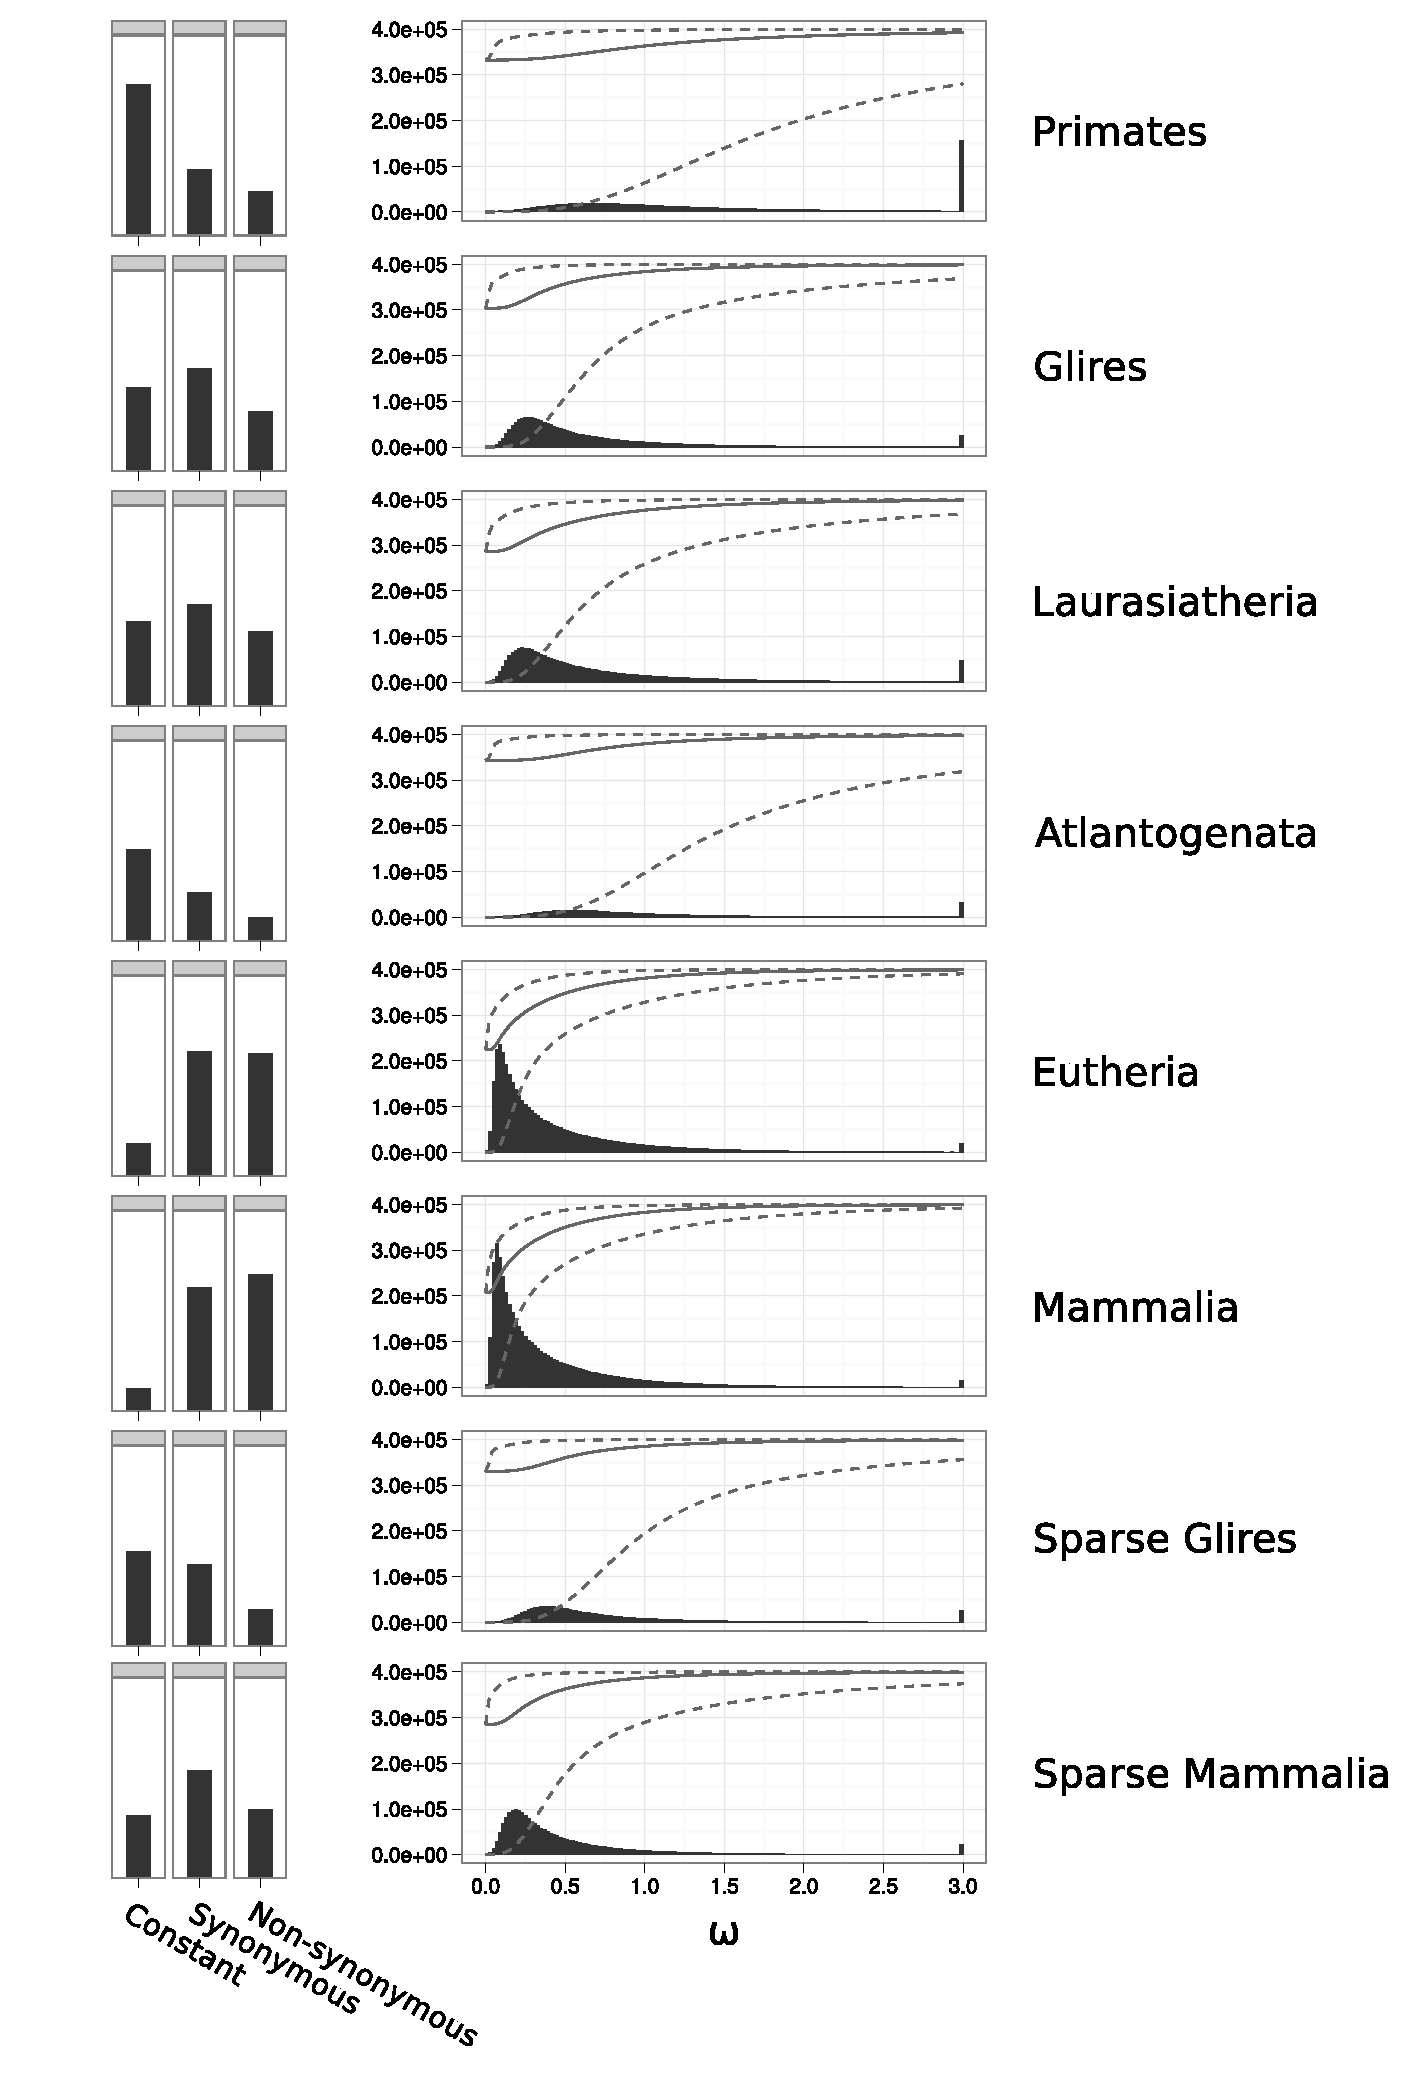
\includegraphics[scale=0.42]{Figs/global_distributions.pdf}
\caption{\scriptsize Global distributions of site patterns and \omg
  estimates for 10 species groups. Left panels: bars represent the
  number of sites showing constant, \syn, and \nsyn patterns. Note,
  the $y$-axis is held constant between rows. Right panels: bars
  represent histograms of \omgml estimates only for sites where
  \omgml$>0$. Sites with \omgml$>0$ correspond to sites with \nsyn
  site patterns, and sites with \omgml$=0$ correspond to constant or
  \syn site patterns. Sites with \omgml$>3$ are counted in the bin at
  \omgml$=3$. A solid line is drawn showing the cumulative
  distribution of \omgml, and dashed lines are drawn above and below
  the solid line showing the cumulative distributions of the lower and
  upper bounds, respectively, of the 95\% confidence interval
  associated with each \sw estimate.}
\label{fig_global_distributions}
\end{figure}

To produce high-confidence \sw estimates across the 10 chosen species
groups, sitewise data from each species group were processed with the
conservative filter as described above. The resulting global
distributions of site patterns, sitewise \omgml estimates, and 95\%
confidence intervals are shown in Figure
\ref{fig_global_distributions}. The left panel in each row shows the
number of sites with constant, \syn, and \nsyn patterns; all sites
with \omgml$=0$ had constant or \syn patterns, and all sites with
\omgml$>0$ had \nsyn patterns. The right panel in each row shows the
distributions of \omgml for sites which contained a \nsyn site
pattern.

The site pattern counts in Figure \ref{fig_global_distributions}
showed that the branch length of each species group had a strong
effect on the overall composition of the sitewise data. Groups
covering little branch length, such as Primates and Atlantogenata,
contained mostly constant sites, while groups covering a large amount
of branch length, such as Eutheria and Mammals, contained few constant
sites and roughly equal proportions of sites with \syn and \nsyn site
patterns.

The distributions of \omgml estimates are shown in Figure
\ref{fig_global_distributions} as a series of histograms showing the
\omgml density (for \nz values of \omgml only) and a series of solid
lines showing the cumulative \omgml density (representing all values);
the lower and upper dashed lines show the cumulative densities of the
lower and upper limits of the 95\% confidence interval resulting from
each \sw estimate. It was clear that the majority of protein-coding
sites have evolved under purifying selection in mammals, a fact which
was most easily seen in the species groups with large total branch
length. The Mammals group showed a maximum density of \nz \omgml
estimates at $\omega\approx0.1$, and the vast majority of sites showed
some evidence of purifying selection with \omgml$<1$.

The \nz \omgml values were more evenly spread in the other species
groups: Glires contained a maximum \nz \omgml density at around
$\omega\approx0.25$ and Primates at $\omega\approx0.7$. This upwards
shift in \nz \omgml estimates relative to Mammals was likely due to
the greater proportion of constant and \syn sites in datasets with
lower overall branch lengths: sites which were truly evolving with
$0<\omega<1$, but where no \nsyn or \syn substitutions were observed,
would have their \omgml estimate ``pushed'' towards zero, presumably
causing an apparent upwards shift in the distribution of the remaining
\nz \omgml values.

\section{Identifying sites with significant evidence for purifying and positive selection}
\label{section_pos_pur}

An important component of SLR's output is \sw information indicating
the confidence with which purifying or positive selection was
detected. These values include the lower and upper bounds of \ci, the
95\% confidence interval for each \omgml estimate, and the LRT
statistic, which corresponds to the strength of evidence for purifying
or positive selection.  sites with \slrt$<0$ showed at least some
evidence for purifying selection, and sites with \slrt$>0$ showed at
least some evidence for positive selection. It should be noted that
the \slrt is a measure of the strength of evidence for purifying or
positive selection, not of the actual strength of that selection. For
example, an alignment covering a very large branch length might yield
a strongly negative \slrt for a site with \omgml only moderately below
1, because the evidence for purifying selection at that site was
highly statistically significant; on the other hand, a
strongly-purifying site in an alignment covering less branch length
might produce a much less-negative \slrt, even with an estimated
\omgml near zero.

\begin{figure}[t!]
\centering
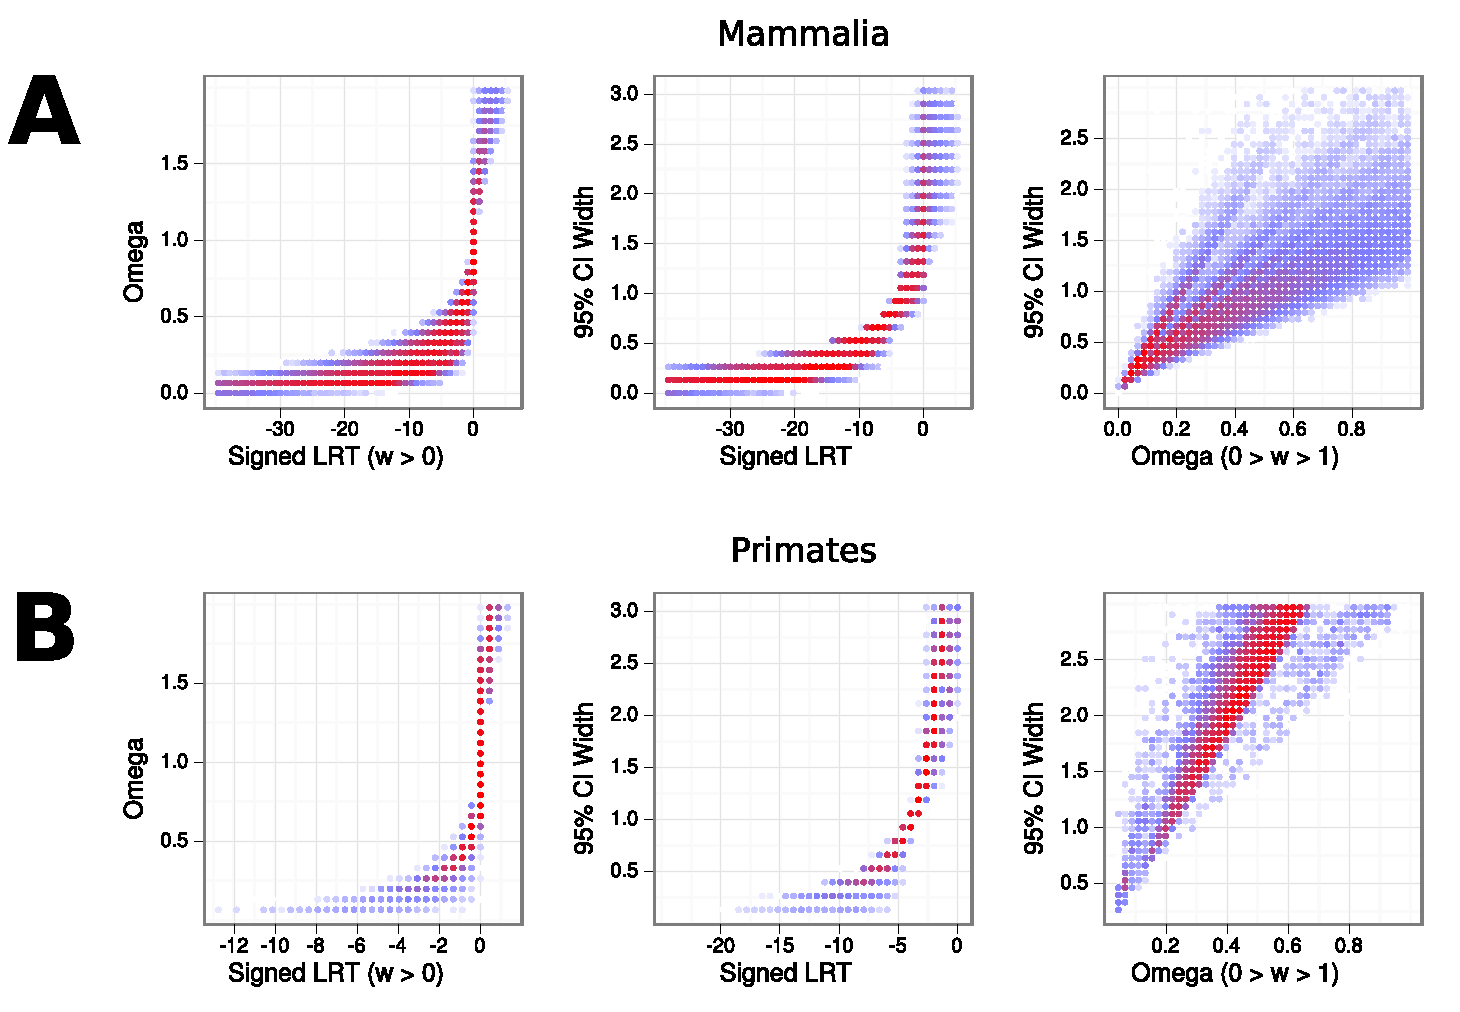
\includegraphics[scale=0.5]{Figs/sites_scatters.pdf}
\caption{The relationship between \slrt, \omgml, and \ci width in (A)
  Mammals and (B) Primates datasets. Each point represents the binned
  density of sites; no points are drawn where no density exists, while
  blue and red points are drawn at areas of low and high density,
  respectively. The left panel shows sites where \omgml$>0$, the
  middle panel shows all sites, and the right panel shows sites where
  $0<$\xspace\omgml$<1.3$. Note the change in $x$-axis scales between plots
  in (A) and (B), reflecting the paucity of sites in Primates with
  strong evidence (\slrt$<$-12) for purifying selection.}
\label{fig_sites_scatters}
\end{figure}

Figure \ref{fig_sites_scatters}A shows the relationship between \slrt,
\omgml and the \ci width for sites from the Mammals group. The left
panel, comparing the \slrt to \nz \omgml estimates, shows that the two
values are highly correlated, with the greatest number of low \omgml
estimates occurring at sites with strongly negative
\slrt. Correspondingly, the middle panel shows an even stronger
relationship between the \slrt magnitude and the \ci width, with the
tightest confidence intervals at sites with very strong evidence for
purifying selection. The rightmost panel compares the \omgml of each
site with the width of its \ci, revealing a more linear and diffuse
positive relationship between \omgml and the size of the \ci. The
equivalent plots for Primates, shown in Figure
\ref{fig_sites_scatters}B, reveal similar patterns, but with generally
less-negative \slrt values, higher \omgml, and larger \ci. These
differences highlight the impact of branch length on the amount of
confidence with which \omg can be estimated on a per-site basis. The
low branch length of the Primates clade rarely yields \omgml estimates
with \ci intervals smaller than 1, while the bulk of sites from the
Mammals dataset have relatively small \ci. Thus, the distribution
of \omgml estimates from datasets with low branch lengths (e.g., the
histogram densities seen in the top few panels of Figure
\ref{fig_global_distributions}) should be interpreted with caution, as
any comparison between \omgml from different sites or datasets may be
more sensitive to the amount of statistical confidence placed on each
estimate than to any meaningful biological difference between the two
sets of data.

\bbtable
\scriptsize{ \centering
\begin{tabular}{lllrrrrrrrrrrrrr}
\toprule
 &  & &  \multicolumn{3}{c}{Site Pattern, \%} & Med. & 
  \multicolumn{3}{c}{Nongap BL} & \multicolumn{2}{c}{\omgml} &
\multicolumn{4}{c}{\omgml Below / Above, \%} \\
\cmidrule(r){4-6} \cmidrule(r){8-10} \cmidrule(r){11-12} \cmidrule(r){13-16}
Name & Filter & Sites & Const. & Syn. & Nsyn. & Codons & Med. & Mean & SD & Mean & SD &
$< 0.5$ & $< 1$ & $> 1$ & $> 1.5$ \\
  \midrule
\input{Tables/pset_summaries_stringent_1.txt}
\bottomrule
\end{tabular}
\caption{\scriptsize Summary statistics of \sw estimates for all
  species groups with the conservative filter applied. Columns under
  the ``\omgml Below / Above'' heading measure the percentage of sites
  with \omgml below or above the indicated value. Med.---median;
  Const.---constant; Syn.---\syn; Nsyn.---\nsyn; BL---branch length; SD---standard deviation.
\label{table_pset_summaries_1}
}

\hspace{.2in}

\centering
\begin{tabular}{llrrrrrrrrrrrrrrrrrrrrr}
\toprule
 & & \multicolumn{8}{c}{Positively Selected Sites (\%)} &
\multicolumn{3}{c}{\chisqlt{0.1}, \%} &
\multicolumn{3}{c}{\chisqlt{0.05}, \%} \\
\cmidrule(r){3-10} \cmidrule(r){7-10} \cmidrule(r){11-13} \cmidrule(r){14-16}
Name & Filter & 
  \multicolumn{2}{c}{\chisqlt{0.1}} & \multicolumn{2}{c}{\chisqlt{0.05}} &
  \multicolumn{2}{c}{\chisqlt{0.01}}& \multicolumn{2}{c}{\bhfdr{0.05}} &
  Neg. & Neut. & Pos. & Neg. & Neut. & Pos. \\
%\cmidrule(r){2-3} \cmidrule(r){4-5} \cmidrule(r){6-7} \cmidrule(r){8-9}
\midrule
\input{Tables/pset_summaries_stringent_2.txt}
\bottomrule
\end{tabular}
\caption{\scriptsize Proportions of sites subject to positive,
  purifying and neutral selection at various \slrt thresholds. The
  method of \citet{Benjamini1995} was used to identify the \slrt
  threshold at which FDR$<$0.05. For columns under the headings
  ``\chisqlt{0.1}, \%'' and ``\chisqlt{0.05}, \%'', Pos. and Neg. are
  the percentage of sites with significant evidence for positive and
  negative selection, respectively, and Neut. is the percentage of
  ``neutral'' sites not showing significant evidence for non-neutral
  selection.}
\label{table_pset_summaries_2}
}
\eetable

Instead, the confidence intervals and \ac{lrt} statistics calculated
by \ac{slr} for each site can be used to identify sites evolving
under purifying or positive selection with confidence. Sites with
\ciup, the upper bound of the \ci interval, below \omg$=1$ could be
interpreted as having evidence of purifying selection with an expected
5\% \fpr; likewise, sites with \cidown above \omg$=1$ contained
evidence of positive selection with an expected 5\% \fpr. In both
cases, \ac{slr} was controlling for an expected 5\% \fpr under the
null model of neutral evolution. As expected, there was a direct
relationship between \ciup and the \chisq approximation to the \slrt
distribution, whereby the set of sites with \ciup$<1$ was exactly
equivalent to the set of sites with \slrt below the negative \chisq
95\% critical value. Similarly, the sites with \cidown$>1$ were those
with \slrt above the \chisq 95\% critical value. Because of this
equality, I will refer to \slrt values at various \chisq threshold
values instead of the 95\% \ci intervals when discussing sites with
significant evidence for purifying or positive selection.

Tables \ref{table_pset_summaries_1} and \ref{table_pset_summaries_2}
provide summaries of the sitewise estimates obtained for each of the
10 mammalian species groups using conservative filtering, showing the
same statistics provided earlier in Tables
\ref{table_filter_summaries_1} and \ref{table_filter_summaries_2} for
the different filters.

Table \ref{table_pset_summaries_2} presents the proportions of
\acp{psc} identified at a variety of \slrt thresholds and in different
species groups, demonstrating that anywhere between 0.01\% to 0.73\%
of sites were identified as under positive selection, depending on the
nominal \ac{fpr} threshold and the species group used.

Different species groups yielded strikingly different estimates of the
proportion of \acp{psc}. At a 5\% \ac{fpr} threshold, the Primates, HQ
Mammals, Laurasiatheria, Eutheria, and Mammals groups produced broadly
comparable proportions of positively-selected sites, ranging from
0.33\% to 0.42\%. The proportions of \acp{psc} in these groups were
higher using a 10\% \ac{fpr} threshold (ranging from 0.46\% to 0.73\%)
and lower using a 1\% \ac{fpr} threshold (ranging from 0.07\% to
0.19\%). When the FDR was controlled using the \citet{Benjamini1995}
method, however, far fewer \acp{psc} were identified. Only the
Eutheria and Mammals groups yielded a substantial number of
positively-selected sites at this level of control; the Primates and
Laurasiatheria data yielded non-zero numbers of \acp{psc} as well, but
these species groups were likely limited in their power to yield
positively-selected sites after FDR control due to their lower total
branch lengths.

The Atlantogenata, HMRD, Sparse Glires, Glires and Sparse Mammals
groups all produced lower proportions of positively-selected sites
identified across all \fpr thresholds. At FDR$<$0.05, all four groups
yielded zero significant \psc{}s, and at a 1\% \ac{fpr} they all
contained lower than 0.01\% \acp{psc}. These species groups were
widely distributed in the amount of total branch length they covered
(ranging in median \ngap branch length from 0.94 for Atlantogenata to
2.55 for Sparse Mammals), suggesting that the lower number of
\acp{psc} was not strongly influenced by branch length; a similar
point could be made of the species groups with higher proportions of
\acp{psc}, which comprised the groups with both the lowest (Primates)
and the highest (Mammals) total branch lengths.

In Mammals, the breakdown of sites into positive, negative and neutral
categories at 10\% and 5\% significance thresholds produced a pattern
similar to that seen in the \omgml distributions from Figure
\ref{fig_global_distributions}. A large amount of purifying constraint
(83.87\% of sites at 5\% FPR), a smaller proportion of
neutrally-evolving sites (15.57\%), and a diminishing fraction of
positively-selected sites (0.55\%) were observed. As expected given
the use of a fixed \slrt threshold to identify purifying sites, the
fraction of sites confidently identified as under purifying selection
showed a strong dependency on the branch length of the species set,
with a much higher power in Mammals than in Primates to confidently
detect purifying selection (83.87\% vs.\ 15.97\%).

The strong correlation between branch length and the amount of
purifying selection detected was consistent with a relatively constant
level of purifying selection in mammalian proteins and greater power
to detect such selection in larger alignments. The overall proportion
of protein-coding sites subject to purifying selection appeared to be
between 90-95\% based on the proportion of sites under purifying
selection with $p<0.1$, \omgml$<0.5$ and \omgml$<1$ (90.61\%, 90.86\%
and 97.25\%, respectively, in Mammals). The effect of branch length
could clearly be seen by comparing the Mammals and Glires species
groups with their ``sparse'' counterparts: in both comparisons, the
proportion of sites with \omgml$<0.5$ was nearly identical, but the
proportion of purifying sites at $p<0.1$ was much lower in the
``sparse'' group.

The detection of positively-selected sites within different species
groups showed no such clear trend. As was perhaps expected, Mammals
and Eutheria, the two species groups with the greatest branch length,
contained the greatest proportion of \acp{psc} at a $p<0.01$
threshold: 0.16\% and 0.19\%, respectively. However, there appeared to
be significant variation---independent of branch length---in the
amount of positive selection detected within different species
groups. Comparing the percentage of \acp{psc} at $p<0.01$ between
Mammals, Sparse Mammals, and HQ Mammals, the ``sparse'' dataset
contained by far the fewest \acp{psc}, and HQ Mammals showed roughly
half as many $p<0.01$ \acp{psc} as Mammals. At a more relaxed $p<0.1$
threshold, HQ Mammals and Mammals contained roughly the same
proportion of \acp{psc}, while Sparse Mammals still had far fewer. The
difference between Mammals and HQ Mammals at the two thresholds
suggested that the larger branch length of the Mammals species group
allowed \acp{psc} to be more readily detected at higher significance
levels. In contrast, the consistently lower proportion of \acp{psc} in
Sparse Mammals could only be readily explained by a species sampling
effect. The Glires and Sparse Glires species groups showed similarly
low levels of positive selection, suggesting that species sampling
within this clade did not strongly affect the prevalence of \acp{psc}.

Despite the large number of species groups considered in this
analysis, it was difficult to assess whether the observed variation in
levels of positive selection was associated with true biological
variation or with some artifact of genome quality or branch
length. With respect to genome quality, the strong presence of
\acp{psc} within the HQ Mammals group provided some evidence that \lcv
genomes were not solely responsible for the increased level of
positive selection in certain species groups. Due to the overlap
between many of the species groups, the effects of branch length and
species sampling were difficult to disentangle. One hypothesis,
motivated by the few \acp{psc} in Sparse Mammals compared to HQ
Mammals, is that a mammalian phylogeny with a greater proportion of
its branch length in shorter or more recent branches may either
contain more positive selection or have more power to detect it. A
thorough exploration of this hypothesis is beyond the scope of this
thesis, but a simple simulation study could be performed to test
whether the \ac{lrt} performed by \ac{slr} is more sensitive to
episodic positive selection occurring within short branches than
within longer branches of the phylogeny.

\section{Synonymous rate variation}

\bresp{Synonymous Rate Variation}

An important concern in the estimation of molecular evolutionary rates
and the detection of positive selection is that the neutral
substitution rate of a DNA sequence can vary significantly depending
on its organismal, chromosomal, or genic context
\citep{Wolfe1987,Gaut1996,Hurst2001,Tuplin2002,Mugal2010}. The most
likely explanation for the observed variation in neutral substitution
rates is some variation in the underlying mutation process, which can
be caused by a number of biological, sequence context, or structural
factors \citep{Ellegren2003,Gaffney2005,Mugal2010}. Accounting for
spatial variation in the neutral mutation rate is of extreme
importance in the inference of natural selection from comparative
sequence data, as the main signal results from the impact of natural
selection on the probability of fixation of non-neutral mutations (see
Chapter \ref{ch_intro}). In the case of detecting non-neutral
evolution in protein-coding regions, the occurrence of synonymous
mutations interleaved with nonsynonymous mutations provides a
convenient source of nearby and putatively neutral mutations which can
be used to estimate a neutral substitution rate. In contrast, the
detection of non-neutral evolution in noncoding elements is fraught
with difficulty in identifying regions from which to estimate a
suitable neutral evolutionary rate \citep{Taylor2008}.

However, some popular methods for detecting sitewise positive
selection assume a constant neutral mutation rate within a given
gene. Although it appears that most mutation rate variation occurs on
a scale of $>$100 kilobases \citep{Gaffney2005} which is greater than
the average gene length, a significant amount of variation still
exists within genes and at individual sites. At sites with high
neutral mutation rates but $\omega\leq1$, both the synonymous and
nonsynonymous substitution rates will be elevated. As a result,
methods which do not model variation in the synonymous substitution
rate may attribute this increase in nonsynonymous substitutions to an
elevated $\omega$ parameter, causing false positive
results. \citet{Pond2005b} described a modified codon model which
allows variation in both the synonymous and nonsynonymous substitution
rates and showed that many genes show significant evidence of
synonymous rate variation. Furthermore, they presented a detailed
analysis of selection in mammalian $\beta$-globin genes, identifying
key differences between sitewise models which account for synonymous
rate variation (termed ``dual'' models) and those which do not (termed
``nonsynonymous'' models).

In light of this evidence for significant synonymous rate variation
within mammalian genes, this section evaluates the potential impact of
synonymous rate variation on the results shown in Tables
\ref{table_pset_summaries_1} and \ref{table_pset_summaries_2}. First,
I undertook a re-analysis of the evidence for positive selection in
$\beta$-globin in mammals to directly compare the sitewise results
from the model of \citet{Pond2005b} with those from recent versions of
PAML and SLR. Second, I examined the genome-wide dataset for
correlations between synonymous substitutions and evidence for
positive selection that might be indicative of a bias due to
synonymous rate variation.

\subsection{Analysis of selection in mammalian $\beta$-globin genes}

\citet{Pond2005b} compared the results of a sitewise Empirical Bayes
analysis of positive selection in mammalian $\beta$-globin genes using
two models: a model based on the M3 model of \citet{Yang2007}, termed
the ``nonsynonymous'' model, and a model with separate parameters for
the nonsynonymous and synonymous evolutionary rates, termed the
``dual'' model. The HyPhy software package \citep{Pond2005} was used
to optimize parameters and calculate likelihoods for both models. I
first attempted to reproduce the results from Table 5 of
\citet{Pond2005b}, using the same alignment and tree and calculating
the Bayes factors for positive selection and the posterior
probabilities of positive selection under four models implemented by
HyPhy: the ``nonsynonymous'' model using either the MG94 or GY94 codon
model specification, and the ``dual'' model using either the MG94 or
GY94 specification. Then, to compare those results to what a typical
user of PAML or SLR might see, I used each of those programs with
their default parameters to estimate sitewise positive selection using
a Bayes Empirical Bayes analysis under the M8 model as implemented by
PAML, and the SLR test as implemented by SLR. Finally, to assess the
impact of the species sampling and data source on these results, I
extracted the equivalent alignment sites from the genome-wide
mammalian dataset used in this chapter and ran the same set of
analyses. Tables \ref{table_syn_rates_hbb_paml} and
\ref{table_syn_rates_hbb_ensembl} present the Bayes factors and
posterior probabilities for $\omega>1$ (for HyPhy analyses), posterior
probability for $\omega>1$ and posterior mean $\omega$ (for the PAML
analysis), or the sitewise LRT, p-value for $\omega>1$, and lower and
upper 95\% confidence intervals for $\omega$ (for the SLR analysis)
for each of the analyses run.

\bbtable
\centering \footnotesize
\begin{tabular}{rrrrrrrrrrrrrrr}
\toprule
 & \multicolumn{8}{c}{HyPhy} & \multicolumn{2}{c}{PAML} & \multicolumn{4}{c}{SLR} \\
 \cmidrule(r){2-9} \cmidrule(r){10-11} \cmidrule(r){12-15}
 & \multicolumn{4}{c}{Nsyn} & \multicolumn{4}{c}{Dual} & \multicolumn{2}{c}{Nsyn} & \multicolumn{4}{c}{--} \\
 \cmidrule(r){2-5} \cmidrule(r){6-9} \cmidrule(r){10-11} \cmidrule(r){12-15}
 & \multicolumn{2}{c}{GY94} & \multicolumn{2}{c}{MG94} & \multicolumn{2}{c}{GY94} & \multicolumn{2}{c}{MG94} 
 & \multicolumn{2}{c}{GY94} & \multicolumn{4}{c}{GY94} \\
\cmidrule(r){1-15}
Site & BF & PP & BF & PP & 
BF & PP & BF & PP & PP & $\omega$ & LRT & pval & $\omega_{low}$ & $\omega_{high}$ \\
  \midrule
\input{Tables/correction_syn_rates_table_yang.txt}
\bottomrule
\end{tabular}
\caption{\scriptsize Evidence for sitewise positive selection in mammalian
  $\beta$-globin using a variety of codon models and mammalian
  alignments from \citet{Pond2005b}. Nsyn---''nonsynonymous'' models,
  which do not model variation in the \syn substitution rate;
  Dual---''dual'' models, which model variation in the \syn
  substitution rate; GY94---a model parameterized using the method of
  \citet{Goldman1994a}; MG94---model parameterized using the method of
  \citet{Muse1994}; BF---Bayes Factor for positive selection;
  PP---posterior probability of positive selection; LRT---likelihood
  ratio test statistic for positive selection.
\vspace*{1 cm}}
\label{table_syn_rates_hbb_paml}


\begin{tabular}{rrrrrrrrrrrrrrr}

\toprule
 & \multicolumn{8}{c}{HyPhy} & \multicolumn{2}{c}{PAML} & \multicolumn{4}{c}{SLR} \\
 \cmidrule(r){2-9} \cmidrule(r){10-11} \cmidrule(r){12-15}
 & \multicolumn{4}{c}{Nsyn} & \multicolumn{4}{c}{Dual} & \multicolumn{2}{c}{Nsyn} & \multicolumn{4}{c}{--} \\
 \cmidrule(r){2-5} \cmidrule(r){6-9} \cmidrule(r){10-11} \cmidrule(r){12-15}
 & \multicolumn{2}{c}{GY94} & \multicolumn{2}{c}{MG94} & \multicolumn{2}{c}{GY94} & \multicolumn{2}{c}{MG94} 
 & \multicolumn{2}{c}{GY94} & \multicolumn{4}{c}{GY94} \\
\cmidrule(r){1-15}
Site & BF & PP & BF & PP & 
BF & PP & BF & PP & PP & $\omega$ & LRT & pval & $\omega_{low}$ & $\omega_{high}$ \\
  \midrule
\input{Tables/correction_syn_rates_table_ensembl.txt}
\bottomrule
\end{tabular}
\caption{\scriptsize Evidence for sitewise positive selection in mammalian
  $\beta$-globin using a variety of codon models and mammalian
  alignments from the genome-wide dataset from this
  thesis. Abbreviations are the same as in Table
  \ref{table_syn_rates_hbb_paml}.}
\label{table_syn_rates_hbb_ensembl}
\eetable

As expected, the results shown in Table \ref{table_syn_rates_hbb_paml}
for the nonsynonymous and dual models implemented by HyPhy
corresponded well with those from Table 5 of \citet{Pond2005b},
displaying strong evidence for positive selection from the
nonsynonymous models at most of the highlighted sites and weaker
evidence from the dual models at a few sites. \citet{Pond2005b}
highlighted codon 85 as a site with a particularly striking difference
between the nonsynonymous and dual models, owing to the high estimated
synonymous rate. Other sites highlighted by the authors were codons 7,
67, and 123. In most of these cases the dual model was in contrast to
the nonsynonymous model, showing non-significant evidence for positive
selection. Although \citet{Pond2005b} did not analyze the difference
between GY94 and MG94 codon models in their $\beta$-globain analysis,
results from the two models are largely in agreement; the main
exceptions are codon 11, where both the nonsynonymous and dual models
yielded a significant result with MG94 but not GY94, and codons 50 and
123, where the dual model yielded significant results with GY94 but
not with MG94.

The PAML M8 and SLR results were similar to the HyPhy nonsynonymous
models at some sites (including codons 7, 50, 67, and 123 where all
four models had PP$>$0.9 or p$<$0.05), but different at others (including
codons 42, 48 and 54, which were strongly significant for all HyPhy
models and non-significant or marginally significant for PAML M8 and
SLR). At codon 85, PAML M8 and SLR yielded non-significant evidence
for positive selection---in agreement with the dual HyPhy model, and
in disagreement with the nonsynonymous HyPhy model. These results
suggest that the detection of positive selection can be dependent both
on the software used and the models underlying the software
implementation. While the lack of explicitly modeling synonymous rate
variation may have led to misleading positive results at some sites,
it appears that the M8 model combined with the Bayes Empirical Bayes
approach suffers less from this problem than does the M3-like
nonsynonymous model as implemented by HyPhy.

Table \ref{table_syn_rates_hbb_ensembl} shows, for comparison, the
same set of analyses performed on the $\beta$-globin alignment from
the genome-wide analysis presented in this chapter. Differences
between corresponding cells in Tables \ref{table_syn_rates_hbb_paml}
and \ref{table_syn_rates_hbb_ensembl} underscore the impact of
different alignment sources and species sampling on the detection of
positive selection; in many cases, the same method yielded significant
evidence in one alignment and insignificant evidence in the other
alignment at the same site (e.g., codon 7 for the GY94 Dual model and
codon 42 for SLR). Overall, the evidence for positive selection at
individual sites seemed stronger in Table
\ref{table_syn_rates_hbb_ensembl}: three codons (42, 50, and 54)
showed significant evidence across all methods tested, while no sites
showed the same result in Table \ref{table_syn_rates_hbb_ensembl}.

Overall, these results suggest that accounting for synonymous rate
variation may be important at sites with elevated long-term mutation
rates, but PAML M8 (using the Bayes Empirical Bayes method) and SLR do
not appear to be as prone to over-confidence at sites with high
synonymous mutation rates as the ``nonsynonymous'' model as
implemented in HyPhy. Further testing using simulation-based
experiments could confirm these observations, but such an analysis is
beyond the scope of this thesis.


\subsection{Genome-wide analysis}

While it was impractical to analybze every gene in as much detail as
presented for $\beta$-globin in the previous subsection, some
assessment of the potential impact of synonymous rate variation on the
sitewise results was warranted. Even if SLR is not strongly biased
towards false positives at sites with high mutation rates, the
analysis of \citet{Pond2005b} showed that synonymous rate variation is
widespread, and some quantification of how many of the
positively-selected sites identified in this chapter might be false
positives due to elevated mutation rates would be helpful in
addressing this concern. Specifically, two questions were asked in the
genome-wide analysis: first, whether SLR showed a general tendency
towards inferring positive selection at sites with a high rate of
synonymous substitution, and second, what proportion of inferred
positively-selected sites showed evidence for an elevated synonymous
rate.

For this analysis, I used the genome-wide inferred ancestral sequences
as in section \ref{section_windows_clustered_subs}, inferring
synonymous and nonsynonymous substitutions along each branch of the
phylogenetic tree at each protein-coding site. Although this approach
was not ideal, as it does not account for multiple substitutions along
a single branch, the lack of very long branches in the Eutherian
phylogenetic tree suggested that this drawback would not severely bias
the results. A more formal approach would involve estimating the
expected counts of synonymous and nonsynonymous substitutions at each
site, but for computational reasons this was not performed.

Using the counts of inferred synonymous and nonsynonymous
substitutions at each site, I first examined the correlation between
SLR's LRT statistic and the counts of synonymous and nonsynonymous
substitutions at each site. Figure \ref{fig_gene_syn_scatter} shows the LRT statistic plotted
against substitution counts for all sites in the $\beta$-globin gene
and \gene{FCRL4}, a glycoprotein member of the immunoglobulin receptor
superfamily. Each codon was categorized as either a purifying,
neutral, or positively-selected site based on the LRT statistic: a LRT
value below the 95\% nominal threshold was considered neutral, and a
LRT value above the 95\% threshold was considered either purifying or
positive depending on the inferred $\omega$ value.

\bbfig
\centering
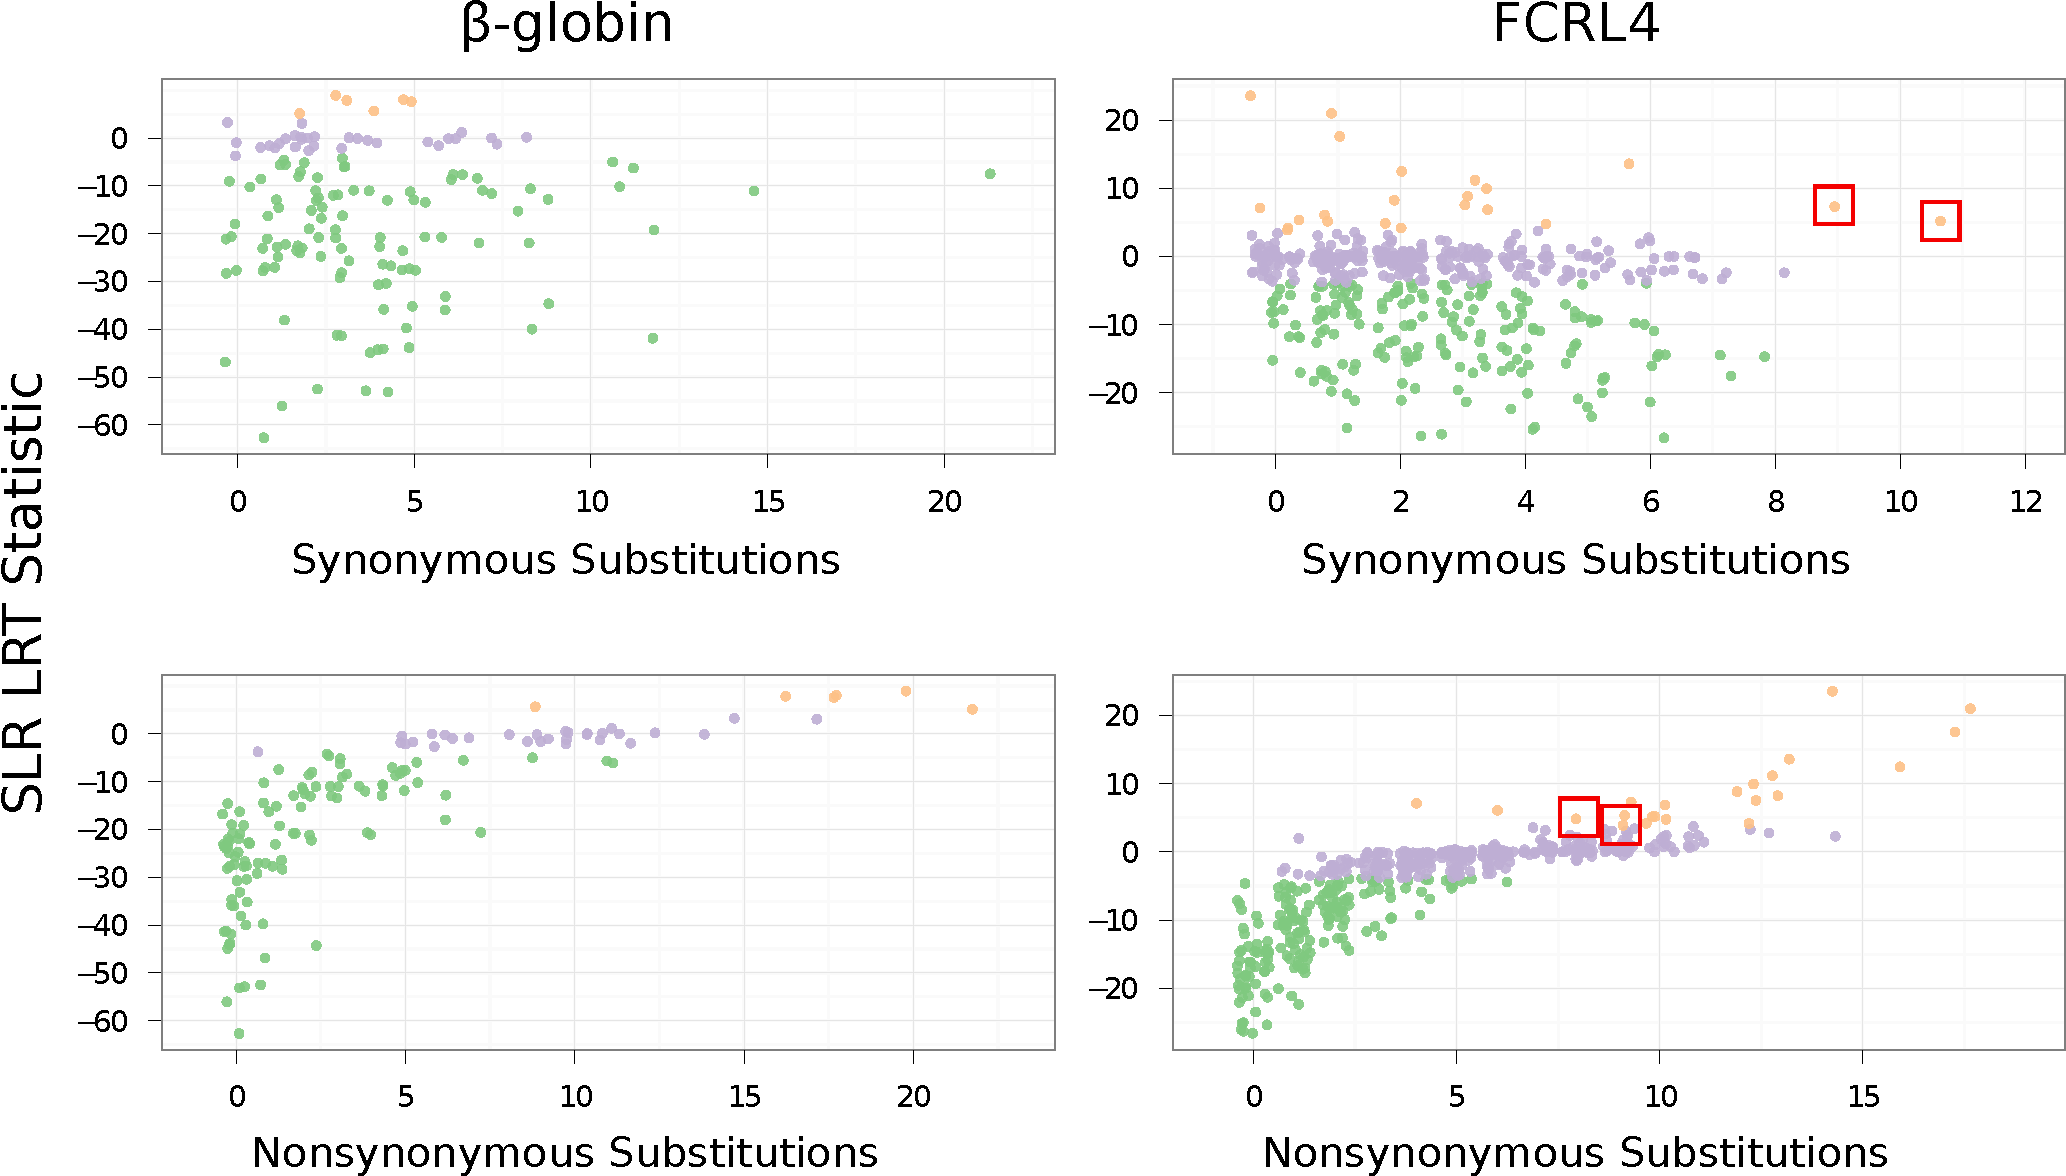
\includegraphics[scale=0.5]{Figs/gene_syn_scatter.pdf}
\caption{Sitewise LRT statistics and synonymous and nonsynonymous
  substitution counts for $\beta$-globin and
  \gene{FCRL4}. Substitution counts were inferred from ancestral
  sequence reconstructions, and sites were categorized based on their
  SLR LRT as purifying (LRT$<-3.84$, green), neutral
  ($-3.84<$LRT$<3.84$, purple), and positive (LRT$>3.84$, orange). Two
  sites with high synonymous substitution counts and LRT$>3.84$ are
  outlined in red. }
\label{fig_gene_syn_scatter}
\eefig

The plot for $\beta$-globin in Figure \ref{fig_gene_syn_scatter} shows
that the variation in SLR's LRT score was driven largely by variation
in nonsynonymous substitutions at each site: all six of the sites
categorized as ``positive'' fell within the middle range of synonymous
substitution counts, but all were at the high end of nonsynonymous
substitution counts. \gene{FCRL4} shows largely the same pattern
except for two sites (highlighted in red) with very high synonymous
rates and only moderate nonsynonymous rates. Sites like these are
candidates for false positives due to a high mutation rate.

In order to identify a suitable cutoff by which to identify sites with
elevated synonymous substitution rates in different genes, the counts
of synonymous and nonsynonymous substitutions at each site were
log-transformed with a pseudocount (i.e., $x = ln(n + 1)$) and
converted into standard z-scores using the following normalization:
$z_{i} = \frac{x_{i} - \mu}{\rho}$ where $\mu$ is the mean of all
log-transformed scores within a gene and $\rho$ is their standard
deviation. (Note that synonymous and non-synonymous z-scores were
calculated separately, and that the log-transformation was found
necessary to better fit the resulting z-scores to a standard normal
distribution.) Figure \ref{fig_zscore_histogram}A shows the
non-log-transformed distribution of z-scores for synonymous
substitution counts, and Figures \ref{fig_zscore_histogram}B and C
show the log-transformed z-scores for synonymous and synonymous
substitution counts, respectively, against the standard normal curve.

\begin{figure}
\centering
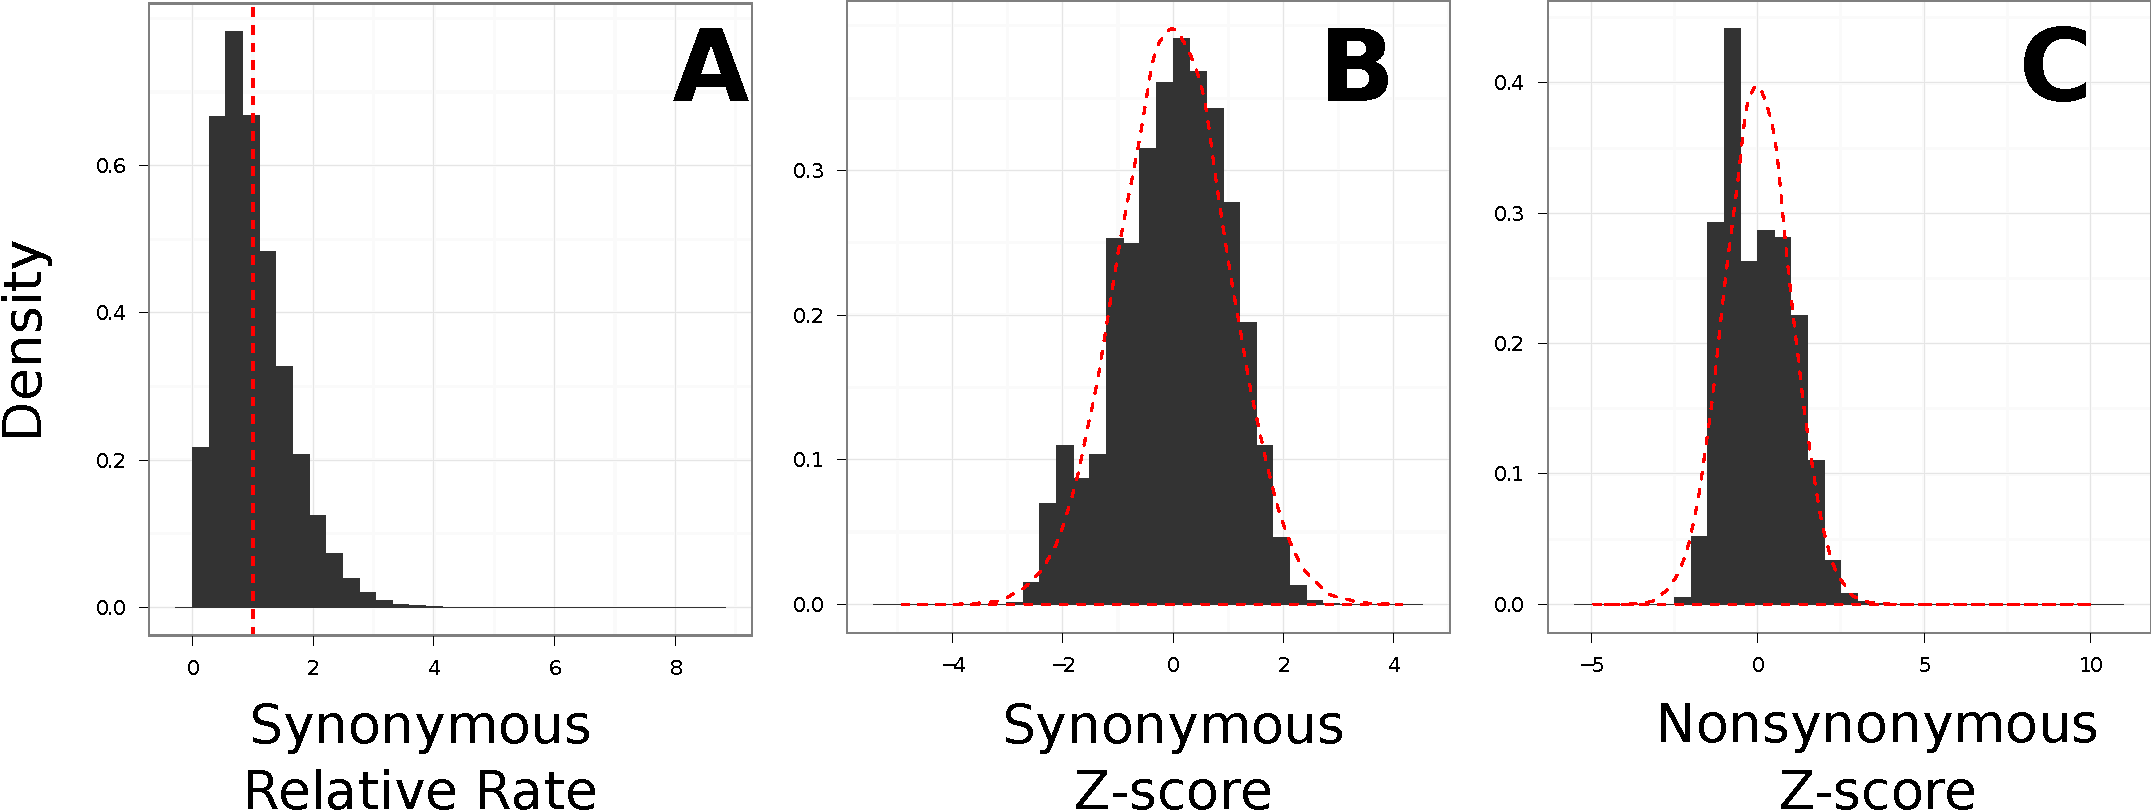
\includegraphics[scale=0.4]{Figs/zscore_histograms.pdf}
\caption{Global distribution of site-wise synonymous and nonsynonymous
  substitution counts. (A) Synonymous relative rates, calculated as
  the synonymous substitution counts divided by the mean synonymous
  substitution count across each gene; a vertical red line is drawn at
  $x=1$. (B) Synonymous z-scores, calculated using log-transformed
  substitution counts as describd in the text; a standard normal
  distribution is shown with a dashed red line. (C) Nonsynonymous
  z-scores, calculated as described in the text; a standard normal is
  shown with a dashed red line.}
\label{fig_zscore_histogram}
\end{figure}


It could be argued that the normalization of synonymous substitution
counts to z-scores is unnecessary and perhaps misleading, as the
z-score is a relative, rather than absolute, measure of an elevated
synonymous rate. Although this section shows results based on the
z-scores, the analysis was performed separately using absolute
synonymous substitution rates compared to the mean (i.e., $z_{i} =
x_{i} / \mu$ where $\mu$ is the mean of all synonymous substitution
counts within a gene) and the results were qualitatively similar. For
reference, 25\% of sites had an absolute synonymous rate of $>$1.31,
10\% had a rate above 1.79, and 5\% above 2.11.

\bbfig
\centering
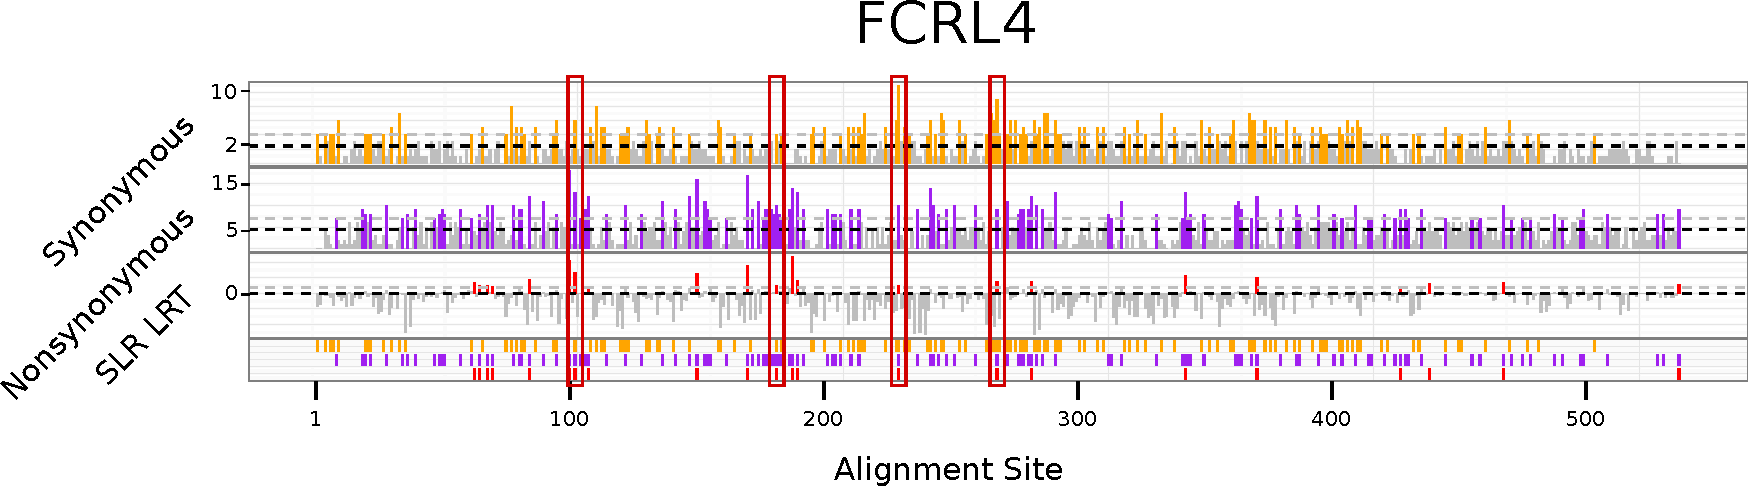
\includegraphics[scale=0.7]{Figs/zscore_sites.pdf}
\caption{Sitewise LRT statistics and synonymous and nonsynonymous
  substitution counts for \gene{FCRL4}. Substitution counts and
  sitewise LRT scores for positive selection were calculated as
  previously described. Sites with synonymous and nonsynonymous
  substitution counts corresponding to the 75\% z-score threshold are
  highlighted in orange and purple, respectively; a dotted black line
  is drawn at the gene-wide mean substitution count and a gray line is
  drawn at the 75\% threshold. Sites with LRT$>3.84$ corresponding to
  the 95\% SLR threshold are highlighted in red; a dotted black line
  is drawn at zero and a gray line is drawn at the 95\%
  threshold. Bottom, colored squares show the co-incidence of sites
  with high synonymous or nonsynonymous substitution counts and
  evidence for positive selection. Sites with evidence for positive
  selection and a high synonymous substitution count are highlighted
  with red rectangles.}
\label{fig_zscore_sites}
\eefig

Figure \ref{fig_zscore_sites} shows the pattern of synonymous
substitution counts, nonsynonymous counts, and SLR LRT scores for
\gene{FCRL4}, with sites corresponding to the 75\% z-score percentile
(z$=0.67$) highlighted in orange (for synonymous substitutions) and
purple (for nonsynonymous substitutions) and sites corresponding to
the 95\% LRT threshold highlighted in red. The bottom row of colored
blocks summarizes the coincidence of positively-selected sites with
high numbers of synonymous or nonsynonymous substitutions, again
showing that most positively-selected sites (except for the codons
highlighted in red) did not show strongly elevated synonymous rates.


To assess whether SLR showed a bias towards identifying positive
selection at sites with high synonymous rates, z-scores were
calculated for sites within the 5,569 genes containing at least one
nominal p$<0.05$ positively-selected site. Three z-score thresholds
(50\%, 75\%, 90\% and 95\%) were used to identify sites with high
synonymous rates, and Fisher's exact test (FET) was used to test for
non-random co-occurrence of positively-selected and high-synonymous
rate sites. The results of this analysis are shown in Table
\ref{table_zscore_tests}, and Figure \ref{fig_zscore_density} shows the
genome-wide distribution of synonymous substitution z-scores
separately for purifying, neutral and positively-selected sites.
Figure \ref{fig_zscore_density} indicates no shift towards elevated
synonymous z-scores for positively-selected sites. Were SLR prone to
identifying positive selection at sites with high synonymous
substitution rates, one would have expected such a shift in
positively-selected compared to neutral and purifying
sites. Furthermore, there appeared to be a genome-wide depletion of
positively-selected sites with high synonymous rates compared to the
random expectation (Fisher's exact test p$=1$, odds ratio 0.49--0.68,
Table \ref{table_zscore_tests}).

\begin{table}
\centering \footnotesize
\begin{tabular}{rrrrrrrrrrrrr}
\toprule
 \multicolumn{2}{c}{Z-score Thresh.} & Mean & \multicolumn{2}{c}{High-Syn. Sites} & \multicolumn{2}{c}{High-Syn. and Pos.} & \multicolumn{3}{c}{FET Results} \\
\cmidrule(r){1-2} \cmidrule(r){4-5} \cmidrule(r){6-7} \cmidrule(r){8-10}
Quantile & Value & Rel. Rate & Count & \% of All & Count & \% of Pos. & Over & Under & OR \\
  \midrule
\input{Tables/zscore_tests.txt}
\bottomrule
\end{tabular}
\caption{Genome-wide overlap between sites with high synonymous
  substitution counts and evidence for positive selection. Synonymous
  rate z-scores were calculated for 3.9 million sites as described in
  the text. Sites with high synonymous rates were identified at
  various thresholds, and 59,801 sites with evidence for positive
  selection were identified using the nominal 95\% LRT threshold. The
  ``Mean Rel. Rate'' column shows the mean relative synonymous rate
  (defined in the text and shown in Figure
  \ref{fig_zscore_histogram}A) for all sites having a z-score above
  the given threshold. The ``High-Syn. Sites'' columns show the count
  and percentage of all sites with a high synonymous rate at the given
  threshold, and the ``High-Syn. and Pos.''  columns show the count of
  sites with both a high synonymous rate and evidence for positive
  selection. The ``Over'' and ``Under'' columns show the p-values for the
  one-tailed Fisher's Exact Test for over- and under-representation,
  respectively, and the ``OR'' column shows the estimated odds ratio.}
\label{table_zscore_tests}
\end{table}


\begin{figure}
\centering
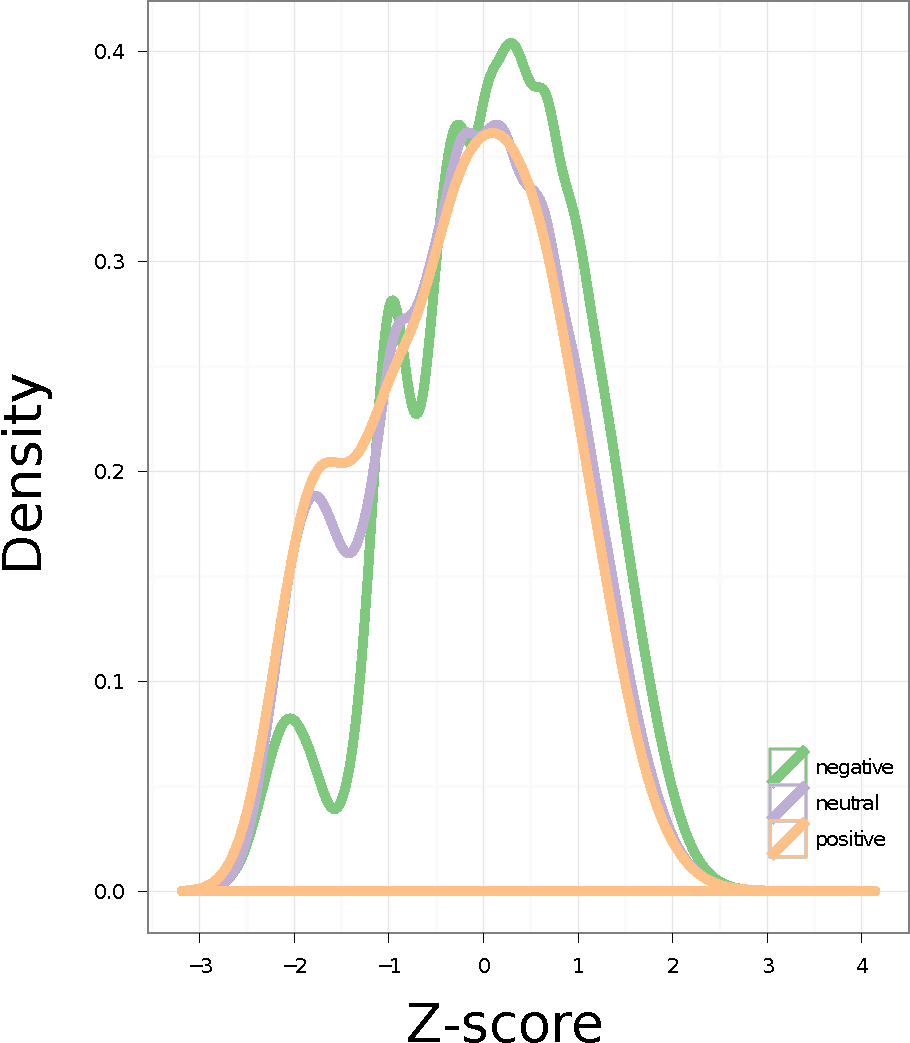
\includegraphics[scale=0.6]{Figs/zscore_density.pdf}
\caption{Global distribution of synonymous count z-scores separated by
  purifying (green), neutral (purple), and positive (orange) sites
  base on the SLR LRT score. Note the under-representation of low
  z-scores at purifying sites (seen in the green curve between z$=-2$
  and z$=-1$): at sites with very few synonymous substitutions, there
  is little data to distinguish between purifying and neutral sites,
  so the magnitude of the LRT score is very low and sites are
  identified as neutral.}
\label{fig_zscore_density}
\end{figure}

Overall, there appeared to be no significant evidence for a strong
impact of synonymous rate variation on the detection of positive
selection using these data. Still, strong variation in the synonymous
substitution rate was observed, and some small proportion of the
positively-selected sites inferred by SLR showed high synonymous
substitution rates. For example, between 1,000 and 5,000 sites (out of
59,000 positively-selected sites and 4 million total sites) contained
synonymous z-scores in the 90-100\% percentile range, indicative of a
very high synonymous substitution rate compared to other sites in the
gene. These sites might reasonably be filtered from a high-confidence
dataset of positively-selected sites. 

\eresp{Synonymous Rate Variation}

\section{The impact of effective population size on protein-coding constraint in mammals}

Another possible source of variation in levels of positive selection
between different species groups was true biological differences in
the proportion of purifying and positively-selected sites. The
conservatively-filtered \sw data showed that, when using \omgml
estimates, between 1\% to 5\% of protein-coding sites are evolving
under positive selection. However, this number varied strongly between
different species groups. Comparing between the four phylogenetically
independent mammalian superorders (Primates, Glires, Laurasiatheria,
and Atlantogenata), Primates showed by far the most \acp{psc} and
sites with \omgml$>1$. Laurasiatheria showed similar proportions of
sites with \omgml$>1$, but Atlantogenata showed fewer \acp{psc} than
Laurasiatheria. The Glires group showed strikingly lower levels of
positive selection compared to the other mammalian
superorders. Despite the relatively large amount of branch length
covered by the Glires group (median total length of 1.77, versus 2.03
for Laurasiatheria), only 0.10\% of sites were identified as \acp{psc}
in Glires at a 5\% \ac{fpr}, compared to 0.33\% in Laurasiatheria and
0.41\% in Primates.

These results may be evaluated in terms of the impact of \ac{ne} on
the efficacy of natural selection in mammals
\citep{Popadin2007,Nikolaev2007,Ellegren2009}. Rodents are known to
have \ac{ne} well above that of primates \citep{Kosiol2008}, and given
the strong correlation between body size, generation time and \ac{ne}
\citep{Nikolaev2007} one can infer that species within the
Laurasiatheria group, with generally longer generation times and
larger body sizes than rodents \citep{Hou2009}, have \ac{ne} more
similar to those seen in primates. The Afrotheria group, containing
species ranging from small moles to elephants and manatees, is more
diverse, making it difficult to estimate an expected historical
\ac{ne}. Nevertheless, Ohta's nearly neutral theory \citep{Ohta1992}
predicts that species with lower \ac{ne} will evolve with less
efficient natural selection. A comparison of the Primates and Glires
data clearly revealed this effect: the proportion of sites with
\omgml~$<0.5$ was 87.27\% for Primates and 90.54\% for Glires. Thus,
differences in the proportion of sites under purifying selection were
well explained by the difference in \ac{ne} between primates and
rodent-like mammals.

Theory also predicts that positive selection should be more efficient
in populations with high \ac{ne} \citep{Ellegren2009,Halligan2010},
and a number of empirical studies have supported this prediction. The
prevalence of adaptive evolution has been extensively studied in
different species using a combination of within-species diversity and
between-species divergence data, finding high proportions of amino
acid substitutions driven by positive selection in species with high
\ac{ne} such as \emph{Drosophila} \citep{Bierne2004} and
\emph{E. coli} \citep{Charlesworth2006}, and low proportions in
species with low \ac{ne} such as human
\citep{Zhang2005b,Sequencing2005a,Boyko2008} and chicken
\citep{Axelsson2009}. Fewer studies have assessed differences in
levels of positive selection between species using only divergence
data and \dnds-based tests for selection, but some such analyses have
been published. \citet{Clark2007} used \acs{paml} \citep{Yang2007} to estimate the
proportion of \acp{psg} and \acp{psc} in 12 \emph{Drosophila} genomes,
finding evidence for positive selection within 33\% of single-copy
orthologs, affecting 2\% of codons within those
\acp{psg}. \citet{Kosiol2008} found a lower proportion of \acp{psg} in
their analysis of 6 mammalian genomes, with only 544 candidate
\acp{psg} out of 16,529 orthologs tested (3.3\%). The authors then
compared the levels of apparent positive selection in different
lineages, finding that 72\% of the 544 candidate \acp{psg} showed
evidence of positive selection in rodents; they concluded that
``whether because of power or a genuine increase in selection, the
rodent branch appears to play a major role in the identification of
PSGs'' \citep{Kosiol2008}. Together, these two studies based on \dnds
estimates largely support the theoretical prediction of increased
levels of positive selection in populations with large \ac{ne}.

The current results appeared to contradict the theoretical prediction
and empirical evidence for a positive correlation between \ac{ne} and
the prevalence of positive selection in mammalian species. The
Primates, Laurasiatheria and HQ Mammals species groups showed greater
levels of positive selection than the Glires group, as measured by
both the proportion of sites with \omgml$>1$ and the proportion of
\acp{psc} identified at all \ac{fpr} and \ac{fdr} thresholds shown in
Table \ref{table_pset_summaries_2}. These species groups were the same
groups which showed evidence for lower long-term \ac{ne} due to their
elevated mean \omgml values and decreased proportion of sites with
\omgml$<1$ (Table \ref{table_pset_summaries_1}). Although estimates of
\omgml should be treated with caution due to stochasticity in the
\ac{ml} estimate at a single alignment site, further evidence for
lower \ac{ne} in these species groups came from the estimates of
gene-wide \dnds values calculated by \ac{slr} based on the M0 codon
model of evolution. Figure \ref{fig_mammals_dnds_ratios} shows a
comparison of gene-wise \dnds in these species groups, providing
strong evidence for the following ordering of \ac{ne}:
Glires~$>$~Laurasiatheria~$\approx$~Atlantogenata~$>$~Primates. Thus,
rather than a positive correlation between \ac{ne} and the prevalence
of positive selection, these \sw data seemed to exhibit a negative
correlation between these two factors.

\begin{figure}[t!]
\centering
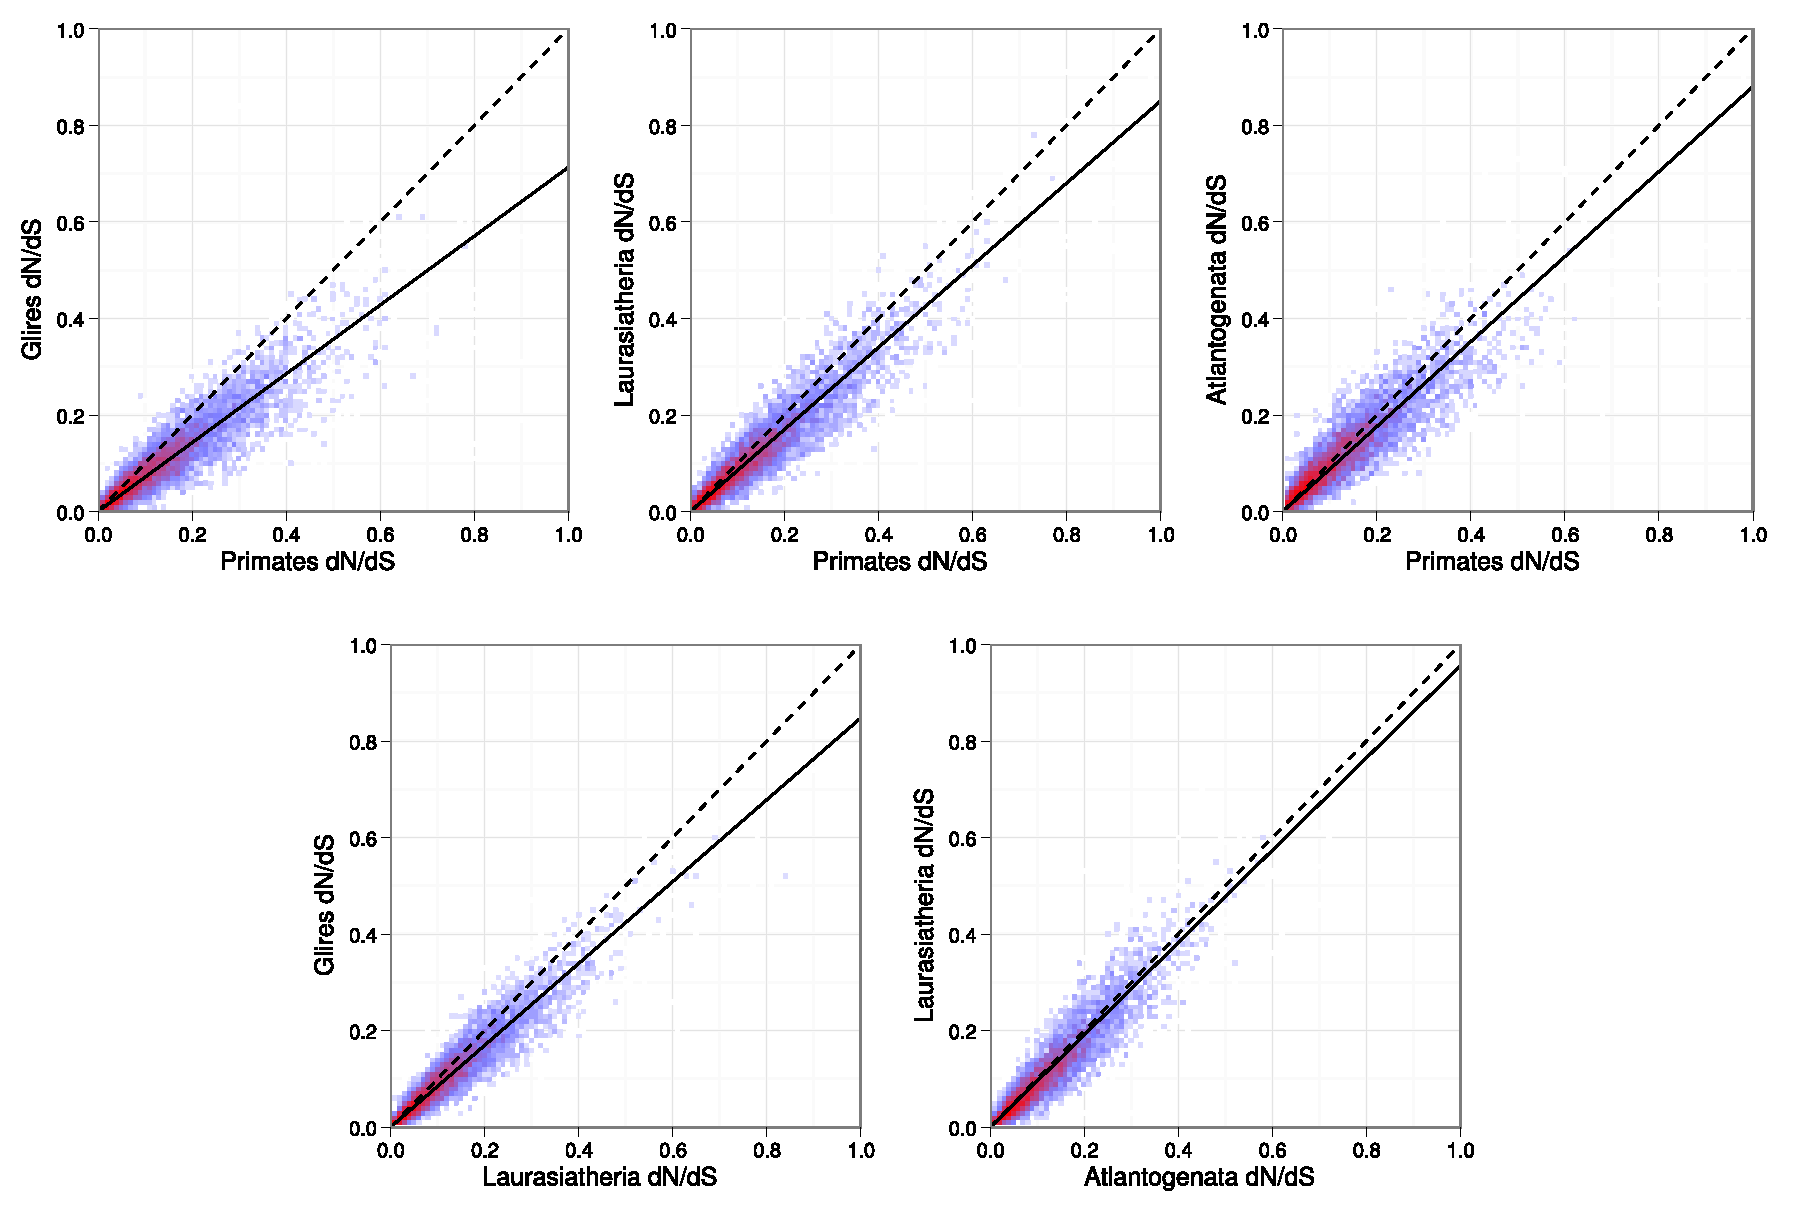
\includegraphics[scale=0.5]{Figs/mammals_dnds_ratios.pdf}
\caption{Correlations between gene-wide \dnds ratios estimated for
  \ntrees orthologous genes in four different species groups. \dnds
  ratios were estimated for each alignment by \ac{slr} using the M0
  (one ratio for all sites) codon model of evolution. Genes were
  plotted according to their \dnds ratio in each species group, and
  each panel shows the density of genes as a colored heat map with red
  areas corresponding to the highest density of points. A dashed line
  with slope of 1 is drawn for reference, and a solid line is drawn in
  each panel along the first principal component axis of those data
  points.}
\label{fig_mammals_dnds_ratios}
\end{figure}

This suggested an alternative interpretation: that perhaps the
different levels of positive selection could be due mainly to the
relaxation of selective constraint in Primates and other species with
low \ac{ne}. A difference in \ac{ne} should impact slightly
deleterious and slightly advantageous mutations equally, with a
greater proportion of both types of mutations being effectively
neutral in the population with lower \ac{ne}. In comparing the
Primates and Glires groups, the expected result was that a subset of
mutations which were under purifying selection in Glires would be
effectively neutral in Primates, bringing the expected \omg for those
sites from $<1$ to 1. The same should occur for slightly advantageous
sites, but if the proportion of slightly deleterious sites is much
greater than the proportion of slightly advantageous sites, it may
have a much more measurable impact. Furthermore, since sites with
\dnds$=1$ are more likely to produce false positive \acp{psc}, it is
plausible that the greater proportion of effectively neutral sites in
a species with low \ac{ne} would lead to an increased proportion of
\acp{psc} detected by methods based on \dnds ratios.

This relaxed constraint argument tempers the interesting observation
of strong differences in the numbers of \acp{psc} between different
species groups. A lower historical \ac{ne} for the Primates and
Laurasiatheria species groups may explain some of the increase in the
number of \acp{psc} detected, even in the absence of true variation in
the prevalence of positive selection between the species groups
investigated here.

Still, the argument may be made that statistical methods for
controlling error rates, such as the \citet{Benjamini1995} method for
FDR control used to identify \acp{psc} at an expected FDR$<0.05$ in
Table \ref{table_pset_summaries_2}, should account for the potential
confounding effects of relaxed constraint noted above. For this
reason, the observation that Primates and Laurasiatheria both yielded
non-zero numbers of \acp{psc} at FDR$<0.05$ may be taken as some
indication of a true difference in the levels of positive selection
between the species groups investigated here. This apparent
discrepancy with previously-published results should be an interesting
area for continued investigation.

\section{Conclusions}

This chapter described the filtering, alignment, and analysis of \sw
selective pressures in a comprehensive set of orthologs across 38
mammalian species. In order to ensure that false signals of positive
selection were avoided as much as possible, several levels of
filtering were applied before and after the estimation of \sw
selective pressures using \ac{slr}: low-quality genomic sequence was
masked out, short or divergent apparent paralogous gene copies were
removed, and alignment columns showing evidence of clustered \nsyn
substitutions or low amounts of evolutionary information were excluded
from the analysis. A comparison of the levels of purifying and
positive selection contained within sites filtered at various
thresholds showed the importance of thorough filtering prior to
genome-wide analysis, highlighting especially the ability of stretches
of mis-annotated or mis-assembled sequence to introduce strong (and
incorrect) signals of localized positive selection. I showed that a
novel approach, based on the identification of lineage-specific
clusters of excessive \nsyn substitutions within short alignment
windows, could effectively target these erroneous regions for removal.

Sitewise selection pressures were then calculated for several groups
of mammalian species. The impact of the total branch length of a
species group on the estimation of \sw selective pressures could be
clearly seen from these results, with the Mammals group containing
many more non-constant alignment sites and a more accurate
distribution of \omgml estimates than groups with little total branch
length, due to the greater amount of evolutionary information.

The \ac{mgp} analysis consortium used the HMRD and HQ Mammals groups
as reference points by which to estimate the increase in power to
detect genome-wide constraint resulting from the additional mammals
sequenced at low coverage. Comparing \sw results to the same reference
species groups, I found that the addition of \lcv genomes increased
the ability to detect purifying constraint in protein-coding regions
by 43.85\% and 136\% compared to the HQ Mammals and HMRD species
groups, respectively, at a 5\% \ac{fpr}. Although I found the levels
of positive selection between species groups to be highly dependent on
the species sampling (and thus, a comparison of ``power'' to be less
meaningful), the Mammals species group identified 21.5\% and 550\%
more \acp{psc} than the HQ Mammals and HMRD species groups,
respectively, at a 5\% \ac{fpr}. Thus, the additional branch length
resulting from the sequencing of \lcv genomes greatly improved the
power to detect purifying and positive selection in mammalian
proteins.

Finally, I analyzed the levels of purifying and positive selection
within four phylogenetically independent mammalian species groups,
identifying strong differences in levels of purifying and positive
selection in different groups, likely resulting from differences in
\ac{ne}. Although the impact of \ac{ne} is well known and has been
previously studied in mammalian species, the work described in this
chapter represented a careful and quantitative analysis of levels of
purifying and positive selection in these species groups. The
observation that the Glires group showed less positive selection than
all other groups suggested a connection between high numbers of
\acp{psc} and relaxed constraint, although Primates and Laurasiatheria
both showed evidence for strong \acp{psc} even at a very stringent FDR
threshold.

More work needs to be done to evaluate what might be causing these
strongly different estimates in different mammalian superorders and to
correctly control for the possible effect of relaxed constraint on the
identification of positive selection in primate genomes. Differences
between the current results and those obtained from diversity-based
estimates in contemporary populations could be attributed to
differences in the timescale under examination \citep{Ellegren2009},
as divergence-based estimates of selective constraint are obviously
sensitive to the long-term \ac{ne} within each clade, while
diversity-based estimates measure the selective constraints based on
more recent \ac{ne}. However, the contrast with the results of
\citet{Kosiol2008}, who used similar \dnds based methods yet found
higher levels of positive selection in the rodent lineage than the
primate lineage, is less easily explained.

An interesting question for future work is whether the observed
species group differences in positive selection result more from
differences in ancient or more recent branches in the phylogeny. In
other words, at what point in evolutionary time did the major
mammalian orders begin to experience different levels of positive
selection (or relaxed constraint)? Although these groups of species
show different contemporary \ac{ne}, they have evolved independently
for several dozen million years, during which time several \ac{ne}
expansions or contractions could have occurred. With more dense
species sampling and branch-specific \dnds estimates, a clearer
picture of the connection between the evolution of \ac{ne}, relaxed
constraint and positive selection may begin to emerge.

\tocite{Eory et al. 2010}{Showed, through constraint analysis of
  various sequence types, that there is higher selective constraint in
  4-fold sites in primates compared to murids. Quote: ``It is well
  established that in several organisms, mutations at 4-fold sites are
  selected against (Chamary et al. 2006; Rocha 2006; Drummond and
  Wilke 2008) and as a consequence the dN/ds ratio, which has been
  frequently used to detect the strength and direction of selection
  (e.g., Dorus et al. 2004; Wang et al. 2006), may be
  underestimated. Our result of higher 4-fold constraint in hominids
  suggests that this bias more strongly affects hominid estimates and
  it may well exceed 20\%.''}

\tocite{Ohta 1993, 1995; Eory et al. 2010}{The Keightley et al. 2011
  paper (ABC to estimate mutation rate parameters) cited Ohta 1993,
  1995 and Eory et al. 2010 for the effective population size and
  efficacy of selection in primates vs.\ murids}

\tocite{Wolf et al. 2009}{Wolf et al. GBE 2009, used pairwise dN dS
  counts to try to show that trends in dN/dS ratios are a result of
  branch length, at least when calculated in a pairwise
  fashion. Slightly unconvincing stuff... could be cited as somehow
  relating to the discussion regarding eff. pop. size, branch length,
  and selection}

\tocite{Berglund et al. 2009}{Berglund et al. 2009 looked at hotspots
  of biased substitutions in humans. Showed that exons with
  accelerated rates in humans have a tendency towards clusters of
  AT-to-GC (weak-to-strong) substitutions. Did some simulations
  showing that this effect is strongest in GC-poor regions, though the
  impact on overall dN/dS is probably minimal (e.g., genes with
  overall high dN/dS didn't show BGC, only the most accelerated exons
  did) and the effect on dN/dS is highest in high-GC regions. The
  most-accelerated exons tend to reside in high-male (but not female)
  recombination, and <50kb from hotspots. Upshot: these biased
  clusters seem to show up in isolated regions (exons), rather than
  spread throughout entire genes. Probably not a huge impact on
  overall apparent constraint.}

\tocite{Duret and Arndt PLoS Gen 2008}{Duret and Arndt 2008 use
  nonreversible nucleotide models to estimate NEUTRAL rates correlated
  with recombination, GC, and GC*. Lots of stuff here, but the
  important bits: overall mutation rate increases with increasing GC
  content (due to overall higher rates of S-W substitution);
  recombination should have a strong impact on W-S substitution, but
  weak impact on S-W substitutions; CpG deamination varies by factor
  of two, very low in GC-poor regions and very high in GC-rich ones.}

\tocite{Galtier et al. TrIG 2009}{Galtier et al. TRIG 2009 is similar
  to Berglund et al. in many ways -- find accelerated exons in a
  primate branch, and identify significantly higher male recombination
  rates there. The number of accelerated exons is small -- ~100 in
  each of four branches -- and not all of these accelerated exons
  showed strongly elevated dN/dS ratios. Only 19 exons at the 1\%
  level. However, they do some nice modeling (mostly in the
  supp. material) which shows that the effect of BCG on dN/dS ratio at
  different GC contents -- it has more effect in GC-rich genes.}

\tocite{Capra and Pollard 2011}{Capra and Pollard quantified BDS
  (biased divergent substitutions) across metazoans, additionally
  using recombination rate data. Dog has the strongest, mouse has the
  weakest BDS scores. (This could be due to lower rec. rate in mouse,
  e.g. Coop and Przeworski 2006)}

\tocite{Nordborg et al. 1996}{Nordborg et al. 1996 (Genet. Res.)
  modeled the effect of background selection on variation in neutral
  linked loci. They showed that weakly selected mutations, rather than
  strongly selected ones, are more likely to produce regional
  patterning of variation in response to local recombination
  rate. Should have a large effect in Drosophila but small effect in
  mammals, though in mammals ``local reductions in regions of reduced
  recombination might be detectable.''}

\tocite{Chun and Fay 2011}{Chun and Fay 2011 (PLoS Gen) looked at
  neutral and deleterious SNP density according to local recombination
  rate, showing that in 'hitchhiking' regions there are fewer neutral,
  but as many deleterious, polymorphisms. That stuff is boring, but
  they also show that the deleterious SNP density stays constant
  throughout the range of recombination rates, while the neutral and
  synonymous SNP density decreases. Thus, slightly deleterious
  mutations are less effectively purged in regions of low
  recombination.}

\tocite{Bullaughey et al. 2008}{Bullaughey et al. (2008, Gen. Res.)
  looked at gene-wide dN/dS ratios in primates and recombination
  rates. They found no significant correlation between broad- or
  fine-scale recomb. rates and rates of protein evolution, **once GC
  content is taken into account**.}

\tocite{SPencer et al. 2006}{Spencer et al. (2006 PLoS Gen) Quote: ``In short,
  while there is a strong relationship between recombination and GC
  content, most of the relationship is explained by scales broader
  than recombination hotspots (16 to 256 kb; unpublished data) and may
  well result from interactions of both factors with additional
  processes such as chromatin organisation or replication
  timing. Similar arguments apply to the question of whether a GC bias
  in recombination-associated mutation can explain the relationship
  between GC content and recombination.''}

